%%%%%%%%%%%%%%%%%%%%%%%%%%%%%%%%%%%%%%%%%%%%%%%%%%%%%%%%%%%%%%%%%%%%%%
% Lớp 11 | Quan hệ vuông góc trong không gian | Hình lăng trụ đứng. Hình chóp đều. Thể tích
% Dạng 1H8?7-2: Thể tích khối chóp tam giác
% Số câu: 72  (sinh tự động bởi tach_cau.py; từ nay thầy sửa trực tiếp file này)
%%%%%%%%%%%%%%%%%%%%%%%%%%%%%%%%%%%%%%%%%%%%%%%%%%%%%%%%%%%%%%%%%%%%%%

%%%%%%%%%%%%%%%% TRẮC NGHIỆM 4 PHƯƠNG ÁN %%%%%%%%%%%%%%%%

% nguồn: Ok_Toan11_TracNghiem_Lan2
\begin{ex}%[1H8N7-2]%[ma:59dc18fe]
	Cho khối chóp $S.ABC$ có chiều cao bằng $5$, đáy $ ABC$ có diện tích bằng $ 6$. Thể tích khối chóp $S.ABC$  bằng
	 \choice
		{$11$} 
		 {\True $10$}
		 {$15$}
		{$30$} 
	 \loigiai{
	$V_{S.ABC}=\dfrac{1}{3}\cdot  S\cdot h=\dfrac{1}{3}\cdot6\cdot5=10$.}
\end{ex}

% nguồn: Ok_Toan11_TracNghiem_Lan2
\begin{ex}%[1H8N7-2]%[ma:203ead9d]
	Cho khối chóp $S.ABC$ có chiều  cao bằng $3$, đáy $ABC$ có diện tích bằng $10$. Thể tích khối chóp $S.ABC$ bằng
	\choice 
		 {$2$}
		{$15$} 
		 {\True $10$}
		{$30$} 
	 \loigiai{
	Thể  tích khối chóp $S.ABC$ là $ V=\dfrac{1}{3}\cdot S\cdot h=\dfrac{1}{3}\cdot10\cdot3=10$.}
\end{ex}

% nguồn: Ok_Toan11_TracNghiem_Lan2
\begin{ex}%[1H8H7-2]%[ma:a0e5539a]
	Cho hình chóp $S.ABC$ có đáy $ABC$ là tam giác đều cạnh $a$. Biết $SA \perp (ABC)$ và  $SA=a\sqrt{3}$. Tính thể tích khối chóp $S.ABC$.
	 \choice
		{\True  $\dfrac{a^3}{4}$}
		 {$\dfrac{a^3}{2}$}
		 {$\dfrac{a^3\sqrt{3}}{4}$}
		 {$\dfrac{3a^3}{4}$}
	\loigiai{ 
		\begin{center}
			\begin{tikzpicture}[scale=1,font=\footnotesize,line join=round,line cap=round,>=stealth]
					\coordinate[label=left:$A$] (A) at  (0,0);
					\coordinate[label=right:$C$] (C) at (3,0); 
					\coordinate[label=below  left:$B$] (B) at (-40:2);
					\coordinate[label=above:$S$] (S) at (90:3); 
					\draw (A)--(B)--(C)--(S)--cycle (S)--(B); 
					 \draw[dashed] (A)--(C);
					\foreach  \diem in {A,B,C,S} \fill (\diem) circle (1pt);
					\draw  pic[draw,angle radius=0.3cm]{right angle=C--A--S};
				\end{tikzpicture}
		\end{center}
		 Đáy là tam giác đều cạnh $a$ nên có diện tích $S_{\triangle ABC} = \dfrac{a^2\sqrt{3}}{4}$.\\
		Chiều cao hình chóp  là $h=SA=a\sqrt{3}$.\\
		Thể  tích khối chóp là
		$$V = \dfrac{1}{3}\cdot S_{\triangle ABC} \cdot SA = \dfrac{1}{3}  \cdot \dfrac{a^2\sqrt{3}}{4} \cdot a\sqrt{3} = \dfrac{a^3}{4}.$$
	} 
\end{ex}

% nguồn: Ok_Toan11_TracNghiem_Lan2
\begin{ex}%[1H8H7-2]%[ma:bc3488c4]
	Cho tứ diện $ABCD$ có $AD$ vuông góc với mặt phẳng $(ABC)$ biết đáy $ABC$ là tam giác vuông tại $B$ và $AD=10$, $AB=10$, $BC=24$. Tính thể tích  của tứ diện $ABCD$.
	 \choice
		 {$V=1200$}
		 {$V=960$}
		{\True $V=400$} 
		{$V=\dfrac{1300}{3}$} 
	\loigiai{ 
		\begin{center}
			\begin{tikzpicture}[scale=1,font=\footnotesize,line join=round,line cap=round,>=stealth]
					\coordinate[label=left:$D$] (D) at  (0,0);
					\coordinate[label=right:$B$] (B) at (4,0); 
					\coordinate[label=below left:$C$] (C)  at (-50:3);
					\coordinate[label=above:$A$] (A) at  (90:4);
					\draw  (D)--(C)--(B)--(A)--cycle (A)--(C);
					\draw[dashed] (D)--(B); 
					\foreach \diem in {D,C,B,A} \fill  (\diem) circle (1pt);
					\draw pic[draw,angle radius=0.3cm]{right  angle=B--D--A};
				\end{tikzpicture}
		\end{center}
		Xem tứ diện là  khối chóp đỉnh $D$ và đáy là tam giác $ABC$.\\
		Chiều cao  của khối chóp là $h=AD=10$.\\
		Diện tích đáy là tam giác vuông $ABC$ 
		$$S_{\triangle ABC}  = \dfrac{1}{2}\cdot AB \cdot BC = \dfrac{1}{2} \cdot 10 \cdot 24 = 120.$$
		Thể tích của tứ  diện là
		$$V = \dfrac{1}{3}\cdot S_{\triangle  ABC} \cdot AD = \dfrac{1}{3} \cdot 120 \cdot 10 = 400.$$
	} 
\end{ex}

% nguồn: Ok_Toan11_TracNghiem_Lan2
\begin{ex}%[1H8H7-2]%[ma:102e30fc]
	Cho khối chóp $S.ABC$ có đáy $ABC$ là tam giác vuông cân tại B,  độ dài cạnh $AB = BC = a$, cạnh bên $SA$ vuông góc với đáy và $SA = 2a$. Tính thể tích $V$ của khối chóp $S.ABC$.
	 \choice
		{\True  $V=\dfrac{a^3}{3}$}
		 {$V=\dfrac{a^3}{2}$}
		{$V=a^3$} 
		 {$V=\dfrac{a^3}{6}$}
	 \loigiai{
		\begin{center}
			\begin{tikzpicture}[scale=1,font=\footnotesize,line join=round,line cap=round,>=stealth]
					\coordinate[label=left:$A$] (A)  at (0,0);
					 \coordinate[label=right:$C$] (C) at (3,0);
					\coordinate[label=below  left:$B$] (B) at (-40:2);
					\coordinate[label=above:$S$] (S) at (90:3); 
					\draw (A)--(B)--(C)--(S)--cycle (S)--(B); 
					 \draw[dashed] (A)--(C);
					\foreach \diem in {A,B,C,S} \fill  (\diem) circle (1pt);
					\draw pic[draw,angle radius=0.3cm]{right angle=C--A--S}; 
				\end{tikzpicture}
		\end{center}
		Chiều cao của khối  chóp là $h=SA=2a$.\\
		Diện  tích đáy là tam giác vuông cân $ABC$
		$$S_{\triangle ABC} = \dfrac{1}{2}\cdot AB \cdot BC =  \dfrac{1}{2}\cdot a \cdot a = \dfrac{a^2}{2}$$
		Thể tích  khối chóp là
		$$V = \dfrac{1}{3}\cdot S_{\triangle ABC} \cdot SA = \dfrac{1}{3} \cdot \dfrac{a^2}{2}  \cdot 2a = \dfrac{a^3}{3}.$$
	 }
\end{ex}

% nguồn: Ok_Toan11_TracNghiem_Lan2
\begin{ex}%[1H8H7-2]%[ma:bbf6020f]
	Cho  hình chóp tứ giác $S.ABCD$ có đáy $ABCD$ là hình vuông cạnh $a$, cạnh bên $SA$ vuông góc với mặt phẳng đáy và $SA=a\sqrt{2}$. Tính thể tích $V$ của khối chóp $S.ABCD$
	 \choice
		 {$V=\dfrac{\sqrt{2}a^3}{6}$}
		 {$V=\dfrac{\sqrt{2}a^3}{4}$}
		{$V=\sqrt{2}a^3$} 
		 {\True $V=\dfrac{\sqrt{2}a^3}{3}$}
	\loigiai{ 
	\immini{Ta có $SA\perp \left(ABCD\right)\Rightarrow  SA$ là đường cao của hình chóp.\\
		Thể tích khối chóp $S.ABCD\colon V=\dfrac{1}{3}SA\cdot  S_{ABCD}=\dfrac{1}{3}\cdot a\sqrt{2}\cdot a^2=\dfrac{a^3\sqrt{2}}{3}$.
		}{	\begin{tikzpicture}[declare function={r=2.5; gocB=-140;}]
		\path  (0,0) coordinate (A)
			(90:r) coordinate (S) 
			(0:r) coordinate (D) 
			(gocB:0.4*r) coordinate (B) 
			($(B)+(D)-(A)$)  coordinate (C);
		\draw  (S)--(D)--(C)--(B)--(S)--(C);
		 \draw[dashed] (S)--(A)--(B)
			(A)--(D); 
		\foreach  \t/\g in {A/160,B/-90,C/-60,S/90,D/0}{
			 \fill[ball color=red] (\t) circle (1pt) node[shift={(\g:7pt)},font=\footnotesize]{$ \t $};
		} 
	\end{tikzpicture}
		} 
	} 
\end{ex}

% nguồn: Ok_Toan11_TracNghiem_Lan2
\begin{ex}%[1H8H7-2]%[ma:ec972cf1]
	Cho khối chóp $S.ABC$ có $SA$ vuông góc với đáy, $SA=4$, $AB=6$, $BC=10$ và $CA=8$. Tính  thể tích $V$ của khối chóp $S.ABC$.
	\choice 
		 {\True $V=32$}
		 {$V=192$}
		{$V=40$} 
		{$V=24$} 
	\loigiai{ 
		\begin{center}
			\begin{tikzpicture}[scale=1,font=\footnotesize,line join=round,line cap=round,>=stealth]
					\coordinate[label=left:$A$]  (A) at (0,0);
					 \coordinate[label=right:$C$] (C) at (3,0);
					\coordinate[label=below left:$B$] (B) at (-40:2); 
					\coordinate[label=above:$S$]  (S) at (90:3);
					 \draw (A)--(B)--(C)--(S)--cycle (S)--(B);
					\draw[dashed]  (A)--(C);
					\foreach \diem  in {A,B,C,S} \fill (\diem) circle (1pt);
					 \draw pic[draw,angle radius=0.3cm]{right angle=C--A--S};
				\end{tikzpicture}
		\end{center}
		Ta có $AB^2+AC^2 = 6^2+8^2 =  100 = BC^2$.\\
		Do đó, tam  giác $ABC$ vuông tại $A$.\\
		Diện tích tam giác $ABC$ là $$S_{\triangle ABC}=\dfrac{1}{2}\cdot AB \cdot AC = \dfrac{1}{2} \cdot  6 \cdot 8 = 24.$$
		 Vì $SA$ vuông góc với đáy nên $SA$ là chiều cao của khối chóp.\\
		Thể tích khối chóp $S.ABC$ là 
		$$V = \dfrac{1}{3}\cdot S_{\triangle ABC} \cdot SA = \dfrac{1}{3} \cdot 24 \cdot 4 = 32.$$ 
	 }
\end{ex}

% nguồn: Ok_Toan11_TracNghiem_Lan2
\begin{ex}%[1H8H7-2]%[ma:4cc91dc0]
	Xét khối chóp tam giác đều cạnh đáy bằng $a$, cạnh bên  bằng 2 lần chiều cao tam giác đáy. Tính thể tích khối chóp.
	\choice 
		{$\dfrac{a^3\sqrt{3}}{2}$} 
		 {$\dfrac{a^3\sqrt{6}}{18}$}
		{\True  $\dfrac{a^3\sqrt{2}}{6}$}
		{$\dfrac{a^3\sqrt{2}}{4}$} 
	\loigiai{ 
	\immini{ 
		Gọi $H$ là trọng tâm tam giác $ABC\Rightarrow SH\perp (ABC)$.\\ 
		Gọi $M$ là trung điểm của cạnh  $BC\Rightarrow AM\perp BC$, $AM=\dfrac{a\sqrt{3}}{2}$.\\
		Do đó $SA=2AM= a\sqrt{3}$.\\ 
		Xét tam giác $SAH$  vuông tại $H$ có $SH=\sqrt{SA^2-AH^2}=\dfrac{2a\sqrt{6}}{3}$.\\
		Vậy $V_{S.ABC}=\dfrac{1}{3}{S_{\Delta ABC}}\cdot SH=\dfrac{1}{3}\cdot \dfrac{a^2\sqrt{3}}{4}\cdot \dfrac{2a\sqrt{6}}{3}=\dfrac{a^3\sqrt{2}}{6}$. 
		}{ 
		\begin{tikzpicture}[scale=1,>=stealth,line join=round,line cap=round,font=\footnotesize]
				\def\a{4} 
				 \def\h{3.5}
				 \def\r{1.5}
				 \def\al{-40}
				\path 
					(0,0)  coordinate (A)
					(\al:\r) coordinate (B) 
					(\a,0) coordinate (C) 
					($(B)!1/2!(C)$) coordinate (M) 
					($(A)!2/3!(M)$)  coordinate (O)
					($(O)$) coordinate  (H)
					($(O)+(0,\h)$) coordinate  (S);
				\draw  (S)--(A)--(B)--(S)--(C)--(B)
					(S)--(M); 
				\draw[dashed,thin]  (A)--(C)
					 (S)--(O)
					(A)--(M); 
				\foreach \p/\g in {A/160,B/-120,C/0,S/90,H/-120,M/-45}\fill (\p) circle  (1pt) node[shift={(\g:.3)}]{$\p$};
				\foreach \a/\b/\c in {S/H/A} 
					{\draw  pic[draw,angle radius=2mm] {right angle = \a--\b--\c};};
			\end{tikzpicture}
		} 
	} 
\end{ex}

% nguồn: Ok_Toan11_TracNghiem_Lan2
\begin{ex}%[1H8H7-2]%[ma:40e459a2]
	Cho  tứ diện $OABC$ có $OA$, $OB$, $OC$ đôi một vuông góc và $OA=OB=OC=a$. Khi đó thể tích của tứ diện $OABC$ là
	\choice 
		 {$V=\dfrac{a^3}{12}$}
		{\True  $V=\dfrac{a^3}{6}$}
		{$V=\dfrac{a^3}{3}$} 
		 {$V=\dfrac{a^3}{2}$}
	\loigiai{ 
		\begin{center}
			\begin{tikzpicture}[scale=1,font=\footnotesize,line join=round,line cap=round,>=stealth]
					\coordinate[label=left:$O$]  (O) at (0,0);
					\coordinate[label=right:$C$] (C) at (4,0); 
					 \coordinate[label=below left:$B$] (B) at (-50:3);
					\coordinate[label=above:$A$] (A) at (90:4); 
					\draw  (O)--(B)--(C)--(A)--cycle (A)--(B);
					\draw[dashed] (O)--(C); 
					\foreach \diem in {O,B,C,A} \fill (\diem) circle  (1pt);
					\draw pic[draw,angle  radius=0.3cm]{right angle=C--O--A};
				\end{tikzpicture}
		\end{center}
		Xem tứ diện là khối chóp đỉnh $A$ và đáy là tam  giác $OBC$.\\
		Vì $OA \perp  OB$ và $OA \perp OC$ nên $OA \perp (OBC)$.\\
		Do đó, chiều cao khối  chóp là $h=OA=a$.\\
		Đáy $OBC$ là tam giác vuông tại $O$. Diện tích đáy  là
		$$S_{\triangle OBC} = \dfrac{1}{2}\cdot OB \cdot OC = \dfrac{1}{2}\cdot a \cdot a  = \dfrac{a^2}{2}.$$
		Thể tích  của tứ diện là
		$$V = \dfrac{1}{3}\cdot S_{\triangle OBC} \cdot OA = \dfrac{1}{3} \cdot \dfrac{a^2}{2} \cdot a =  \dfrac{a^3}{6}.$$
	} 
\end{ex}

% nguồn: Ok_Toan11_TracNghiem_Lan2
\begin{ex}%[1H8H7-2]%[ma:744fa351]
	Hình chóp tam giác đều $S.ABC$ có cạnh đáy là $a$ và  mặt bên tạo với đáy góc $45^\circ $. Tính theo $a$ thể tích khối chóp $S.ABC$.
	 \choice
		{$\dfrac{a^3}{8}$} 
		{\True  $\dfrac{a^3}{24}$}
		{$\dfrac{a^3}{12}$} 
		 {$\dfrac{a^3}{4}$}
	 \loigiai{
	 \immini
		{ 
		 Gọi $G$ là tâm của tam giác đều $ABC$ và $M$ là trung điểm $BC$.\\
		Theo giả thiết góc giữa mặt bên và đáy  bằng $45^\circ$ suy ra $\widehat{SMG}=45^\circ$.\\
		Tam giác $ABC$ đều  cạnh $a$ nên $AM=\dfrac{\sqrt{3}}{2}a$ và $GM=\dfrac{1}{3}AM=\dfrac{a\sqrt{3}}{6}$.\\
		Xét tam giác $SGM$  có $$\tan\widehat{SMG}=\dfrac{SG}{GM}\Rightarrow\tan 45^\circ=\dfrac{SG}{GM}\Rightarrow SG=GM=\dfrac{a\sqrt{3}}{6}.$$
		Vậy thể tích khối  chóp $S.ABC$ là $$V_{S.ABC}=\dfrac{1}{3}{S_{ABC}}\cdot SG=\dfrac{1}{3}\cdot \dfrac{\sqrt{3}}{4}{a^2}\cdot \dfrac{a\sqrt{3}}{6}=\dfrac{a^3}{24}.$$
		} 
		 {
		\begin{tikzpicture}[>=stealth,line join=round,line cap=round,font=\footnotesize,scale=0.7]
				 \def\h{4}
				 \coordinate[label=left:{$A$}] (A) at (0,0);
				\coordinate[label=below:{$B$}] (B) at (1.7,-1.75); 
				 \coordinate[label=right:{$C$}] (C) at (5,0);
				\coordinate[label=below right:{$M$}] (M)  at ($(B)!0.5!(C)$);
				\coordinate[label=below:{$G$}] (G)  at ($(A)!2/3!(M)$);
				\coordinate[label=above:{$S$}] (S) at ($(G)+(0,\h)$); 
				\draw (S)--(A)--(B)--(C)--cycle (S)--(B) 
					 (S)--(M);
				 \draw[dashed] (A)--(C)
					 (A)--(M)
					 (S)--(G);
				\foreach \p in  {A,B,C,S,G,M}
				\fill (\p)  circle (1pt);
				 \pic[draw,angle radius=3.5mm,angle eccentricity=1.5] {angle = S--M--A};
			\end{tikzpicture}
		 }
	 }
\end{ex}

% nguồn: Ok_Toan11_TracNghiem_Lan2
\begin{ex}%[1H8H7-2]%[ma:5d4c1b11]
	Cho khối chóp $S.ABC$ có  đáy $ABC$ là tam giác cân tại $A$ với $BC=2a$, $\widehat{BAC}=120^\circ $, biết $SA\perp (ABC)$ và mặt $(SBC)$ hợp với đáy một góc $45^\circ$. Tính thể tích khối chóp $S.ABC$.
	\choice 
		{$\dfrac{a^3}{2}$} 
		 {$a^3\sqrt{2}$}
		 {\True $\dfrac{a^3}{9}$}
		{$\dfrac{a^3}{3}$} 
	\loigiai{ 
	 \immini
		{ 
		Gọi $I$ là trung điểm  $BC$.\\
		Do $\Delta ABC$ cân tại  $A$ nên $BC\perp AI$.\\
		 Mặt khác do $SA\perp (ABC)\Rightarrow BC\perp SA$.\\
		Suy ra $BC\perp SI$.\\ 
		Do  đó góc giữa $(SBC)$ và đáy chính là góc $\widehat{SIA}=45^\circ $.\\
		Xét $\Delta AIB$ vuông tại $I$ có $IB=a$, $\widehat{IAB}=60^\circ$,\\ suy ra  $IA=\dfrac{IB}{\tan 60^\circ}=\dfrac{a}{\sqrt{3}}$.
		 }
		 {
		\begin{tikzpicture}[font=\footnotesize,line cap=round,line join=round,>=stealth,x=1.0cm,y=1.0cm,scale=0.5]
				 \path
					(-2.3,0.61) coordinate  (A)
					(1.92,-1.71) coordinate  (B)
					 (4.23,0.61) coordinate (C)
					(-2.3,6.01) coordinate (S) 
					(3.08,-0.55)  coordinate (I);
				\draw (S)--(A) 
					(S)--(B) 
					 (S)--(C)
					(S)--(I) 
					 (B)--(C)
					(A)--(B) 
					 (B)--(C);
				\draw[dashed]  (A)--(C)
					(A)--(I); 
				 \foreach \x/\g in{A/-130,B/-100,C/-80,S/90,I/-50}
				\fill(\x) circle  (1pt)
					 ($(\x)+(\g:5mm)$) node{\small $\x$};
				\draw  pic[angle radius=6pt,angle eccentricity=1.5] {angle = S--I--A};
			\end{tikzpicture}
		} 
		 \noindent
		Xét $\Delta SAI$ vuông tại $A$  có $IA=\dfrac{a}{\sqrt{3}}$, $\widehat{SIA}=45^\circ $ nên $\Delta SAI$ vuông cân tại $A$,\\do đó $SA=IA=\dfrac{a}{\sqrt{3}}$.\\
		Thể tích của  khối chóp $S.ABC$ là $$V=\dfrac{1}{3}{S_{\Delta ABC}}\cdot SA=\dfrac{1}{3}\cdot \dfrac{1}{2}BC\cdot AI\cdot SA=\dfrac{a^3}{9}.$$
	 }
\end{ex}

% nguồn: Ok_Toan11_TracNghiem_Lan2
\begin{ex}%[1H8H7-2]%[ma:05bad2bd]
	Cho một hình chóp tam giác đều có cạnh đáy bằng $a$, góc giữa cạnh bên và mặt phẳng đáy bằng $45^\circ$. Thể tích khối chóp đó là 
	 \choice
		{$\dfrac{a^3\sqrt{3}}{12}$} 
		{\True $\dfrac{a^3}{12}$} 
		 {$\dfrac{a^3}{36}$}
		 {$\dfrac{a^3\sqrt{3}}{36}$}
	 \loigiai{
	\immini{ 
		 Gọi $O$ là trọng tâm tam giác $ABC$, ta có $SO\perp(ABC)$.\\
		Suy  ra $\left(SA,(ABC)\right)=\widehat{SAO}=45^\circ$.\\
		 Ta có $SO=AO\cdot \tan 45^\circ =\dfrac{a\sqrt{3}}{3}$.\\
		Vậy $V=\dfrac{1}{3}  SO\cdot{S_{ABC}}=\dfrac{1}{3}\cdot \dfrac{a\sqrt{3}}{3}\cdot \dfrac{a^2\sqrt{3}}{4}=\dfrac{a^3}{12}$.
		}{ 
		\begin{tikzpicture}[scale=1,>=stealth,line join=round,line cap=round,font=\footnotesize]
				\def\a{4} 
				\def\h{3.5} 
				 \def\r{1.5}
				\def\al{-40} 
				\path 
					(0,0)  coordinate (A)
					(\al:\r) coordinate  (B)
					(\a,0) coordinate  (C)
					 ($(B)!1/2!(C)$) coordinate (M)
					($(A)!2/3!(M)$)  coordinate (O)
					 ($(O)+(0,\h)$) coordinate (S);
				\draw (S)--(A)--(B)--(S)--(C)--(B) 
					(S)--(M); 
				\draw[dashed,thin]  (A)--(C)
					 (S)--(O)
					 (A)--(M);
				\foreach \p/\g in {A/160,B/-120,C/0,S/90,O/-120,M/-45}\fill  (\p) circle (1pt) node[shift={(\g:.3)}]{$\p$};
				\foreach \a/\b/\c in  {S/O/A}
					{\draw pic[draw,angle radius=2mm] {right angle  = \a--\b--\c};};
			\end{tikzpicture}
		 }
	 }
\end{ex}

% nguồn: Ok_Toan11_TracNghiem_Lan2
\begin{ex}%[1H8H7-2]%[ma:dbbf1f19]
	Cho hình chóp tam giác đều $S.ABC$ có  cạnh đáy bằng $2a$, cạnh bên tạo với đáy một góc $60^\circ$. Thể tích khối chóp $S.ABC$ là
	\choice 
		 {\True $\dfrac{2a^3\sqrt{3}}{3}$}
		 {$\dfrac{a^3\sqrt{3}}{3}$}
		 {$\dfrac{a^3\sqrt{3}}{4}$}
		 {$a^3\sqrt{3} $}
	\loigiai{ 
	\immini{ 
		Gọi $O$ là tâm  đường tròn ngoại tiếp $\Delta ABC$ thì $SO\perp (ABC)$.\\
		Suy  ra $\widehat{SAO}=60^\circ $.\\
		Ta có $AO=\dfrac{2}{3}\cdot 2a\cdot \dfrac{\sqrt{3}}{2}=\dfrac{2a\sqrt{3}}{3}$, $SH=AO\cdot\tan  60^\circ=2a$.\\
		Diện tích $\Delta  ABC$ là $S_{ABC}=\dfrac{(2a)^2\cdot \sqrt{3}}{4}=a^2\sqrt{3}$.\\
		Thể tích khối chóp $S.ABC$ là $$V=\dfrac{1}{3}{S_{ABC}}\cdot  SO=\dfrac{2a^3\sqrt{3}}{3}.$$
		}{ 
		\begin{tikzpicture}[font=\footnotesize,line join=round,line cap=round,>=stealth]
				\path 
					(0,0) coordinate  (A)
					(1.8,-2.5) coordinate  (B)
					(5,0) coordinate (C) 
					($(B)!0.5!(C)$) coordinate  (M)
					($(A)!.6667!(M)$) coordinate (O) 
					($(O)+(0,3.5)$) coordinate (S); 
				\draw  (S)--(B)--(C)--(S)--(A)--(B);
				\draw[dashed] (C)--(A)--(M)  (S)--(O);
				 \foreach \x/\g in{A/180,B/-90,C/0,M/-45,O/-90,S/90}
				\fill(\x) circle  (1pt)
					($(\x)+(\g:4mm)$)  node{$\x$};
			\end{tikzpicture}
		} 
	 }
\end{ex}

% nguồn: Ok_Toan11_TracNghiem_Lan2
\begin{ex}%[1H8H7-2]%[ma:dbe66898]
	Cho hình chóp $S.ABC$ có đáy là tam giác đều cạnh $a$, cạnh bên $SA$ vuông góc với đáy và thể tích của  khối chóp đó bằng $\dfrac{a^3}{4}$. Tính cạnh bên $SA$.
	\choice 
		{$\dfrac{a\sqrt{3}}{2}$} 
		 {$\dfrac{a\sqrt{3}}{3}$}
		{\True  $a\sqrt{3}$}
		 {$2a\sqrt{3}$}
	\loigiai{ 
		\begin{center}
			\begin{tikzpicture}[scale=1,font=\footnotesize,line join=round,line cap=round,>=stealth]
					 \coordinate[label=left:$A$] (A) at (0,0);
					\coordinate[label=right:$C$] (C)  at (3,0);
					\coordinate[label=below left:$B$] (B) at (-40:2); 
					\coordinate[label=above:$S$]  (S) at (90:3);
					\draw  (A)--(B)--(C)--(S)--cycle (S)--(B);
					 \draw[dashed] (A)--(C);
					\foreach  \diem in {A,B,C,S} \fill (\diem) circle (1pt);
					\draw  pic[draw,angle radius=0.3cm]{right angle=C--A--S};
				\end{tikzpicture}
		\end{center}
		Diện tích đáy là tam giác đều cạnh  $a$ là $S_{\triangle ABC} = \dfrac{a^2\sqrt{3}}{4}$.\\
		Thể tích khối chóp là $V = \dfrac{1}{3}\cdot S_{\triangle ABC} \cdot SA$. 
		Suy  ra
		$$SA = \dfrac{3\cdot V}{S_{\triangle ABC}} = \dfrac{3 \cdot  \dfrac{a^3}{4}}{\dfrac{a^2\sqrt{3}}{4}} = a\sqrt{3}.$$
	} 
\end{ex}

% nguồn: Ok_Toan11_TracNghiem_Lan2
\begin{ex}%[1H8H7-2]%[ma:771b1076]
	Cho hình chóp $S.ABC$ có cạnh bên $SA$ vuông góc với mặt phẳng đáy $(ABC)$. Biết $SA=a$, tam giác $ABC$ là tam giác vuông cân tại $A$, $AB=2a$. Tính theo $a$ thể tích  $V$ của khối chóp $S.ABC$.
	 \choice
		{$V=\dfrac{a^3}{6}$} 
		{$V=\dfrac{a^3}{2}$} 
		 {\True $V=\dfrac{2a^3}{3}$}
		{$V=2a^3$} 
	\loigiai{ 
		\begin{center}
			\begin{tikzpicture}[scale=1,font=\footnotesize,line join=round,line cap=round,>=stealth]
					\coordinate[label=left:$A$] (A)  at (0,0);
					\coordinate[label=right:$C$] (C) at (3,0); 
					\coordinate[label=below left:$B$] (B)  at (-40:2);
					\coordinate[label=above:$S$] (S) at (90:3); 
					\draw (A)--(B)--(C)--(S)--cycle  (S)--(B);
					 \draw[dashed] (A)--(C);
					\foreach \diem in  {A,B,C,S} \fill (\diem) circle (1pt);
					\draw pic[draw,angle radius=0.3cm]{right  angle=C--A--S};
				\end{tikzpicture}
		\end{center}
		Chiều cao của  khối chóp là $h=SA=a$.\\
		Đáy $ABC$  là tam giác vuông cân tại $A$ nên $AC = AB = 2a$.\\
		Diện tích  đáy là
		$$S_{\triangle ABC} = \dfrac{1}{2}\cdot AB \cdot AC = \dfrac{1}{2}\cdot2a\cdot 2a =  2a^2.$$
		 Thể tích của khối chóp là
		$$V =  \dfrac{1}{3}\cdot S_{\triangle ABC} \cdot SA = \dfrac{1}{3} \cdot 2a^2 \cdot a = \dfrac{2a^3}{3}.$$
	} 
\end{ex}

% nguồn: Ok_Toan11_TracNghiem_Lan2
\begin{ex}%[1H8H7-2]%[ma:03da4389]
	Cho khối chóp tam giác  đều $S.ABC$ có cạnh đáy bằng $a$ và cạnh bên bằng $2a$. Tính thể tích $V$ của khối chóp $S.ABC$.
	\choice 
		{$V=\dfrac{\sqrt{11}a^3}{6}$} 
		{$V=\dfrac{\sqrt{11}a^3}{4}$} 
		 {$V=\dfrac{\sqrt{13}a^3}{12}$}
		{\True $V=\dfrac{\sqrt{11}a^3}{12}$} 
	 \loigiai{
		\begin{center}
			\begin{tikzpicture}[scale=1,font=\footnotesize,line join=round,line cap=round,>=stealth]
					 \coordinate[label=left:$A$] (A) at (0,0);
					\coordinate[label=right:$C$]  (C) at (3.5,0);
					\coordinate[label=below left:$B$] (B) at (-65:2.5); 
					\coordinate[label=below right:$M$] (M) at  ($(B)!.5!(C)$);
					 \coordinate[label=below:$O$] (O) at ($(A)!2/3!(M)$);
					\coordinate[label=above:$S$] (S)  at ($(O)+(90:3.5)$);
					\draw  (A)--(B)--(C)--(S)--cycle (S)--(B);
					 \draw[dashed] (M)--(A)--(C)
						 (O)--(S);
					\foreach \diem  in {A,B,C,M,O,S} \fill (\diem) circle (1pt);
					\draw pic[draw,angle  radius=0.3cm]{right angle=M--O--S};
				\end{tikzpicture}
		\end{center}
		Gọi $O$  là trọng tâm của tam giác đều $ABC$.\\
		Vì $S.ABC$ là chóp tam giác đều nên $SO \perp (ABC)$ và $SO$ là  chiều cao của khối chóp.\\
		 Đáy là tam giác đều nên diện tích đáy là
		$$S_{\triangle  ABC} = \dfrac{a^2\sqrt{3}}{4}.$$
		Gọi $M$ là trung điểm $BC$, ta có  đường cao của đáy là $AM = \dfrac{a\sqrt{3}}{2}$.\\
		Vì $O$ là trọng  tâm nên $AO = \dfrac{2}{3}\cdot AM = \dfrac{2}{3} \cdot \dfrac{a\sqrt{3}}{2} = \dfrac{a\sqrt{3}}{3}$.\\
		Xét tam giác $SOA$ vuông tại $O$, ta có 
		$$SO = \sqrt{SA^2 - AO^2}  = \sqrt{(2a)^2 - \left(\dfrac{a\sqrt{3}}{3}\right)^2} = \sqrt{4a^2 - \dfrac{a^2}{3}} = \dfrac{a\sqrt{33}}{3}.$$
		Thể tích khối chóp là 
		$$V = \dfrac{1}{3}\cdot S_{\triangle ABC} \cdot SO = \dfrac{1}{3}  \cdot \dfrac{a^2\sqrt{3}}{4} \cdot \dfrac{a\sqrt{33}}{3} = \dfrac{a^3\sqrt{11}}{12}.$$
	} 
\end{ex}

% nguồn: Ok_Toan11_TracNghiem_Lan2
\begin{ex}%[1H8H7-2]%[ma:62a3eee0]
	Cho hình chóp $S.ABC$ có đáy là tam  giác đều cạnh $a$. Cạnh bên $SC$ vuông góc với mặt phẳng $(ABC)$, $SC=a$. Thể tích khối chóp $S.ABC$ bằng
	 \choice
		{$\dfrac{a^3\sqrt{3}}{3}$} 
		{\True  $\dfrac{a^3\sqrt{3}}{12}$}
		 {$\dfrac{a^3\sqrt{3}}{9}$}
		 {$\dfrac{a^3\sqrt{3}}{12}$}
	\loigiai{ 
		\begin{center}
			\begin{tikzpicture}[scale=1,font=\footnotesize,line join=round,line cap=round,>=stealth]
					 \coordinate[label=left:$A$] (A) at (0,0);
					\coordinate[label=right:$C$] (C) at (3,0); 
					\coordinate[label=below  left:$B$] (B) at (-40:2);
					\coordinate[label=above:$S$] (S) at (90:3); 
					 \draw (A)--(B)--(C)--(S)--cycle (S)--(B);
					\draw[dashed] (A)--(C); 
					 \foreach \diem in {A,B,C,S} \fill (\diem) circle (1pt);
					\draw pic[draw,angle radius=0.3cm]{right angle=C--A--S}; 
				\end{tikzpicture}
		\end{center}
		Đáy là tam  giác đều cạnh $a$ nên có diện tích $S_{\triangle ABC} = \dfrac{a^2\sqrt{3}}{4}$.\\
		Chiều  cao hình chóp là $h=SC=a$.\\
		Thể tích khối chóp  là
		$$V = \dfrac{1}{3}\cdot S_{\triangle ABC} \cdot SC = \dfrac{1}{3} \cdot \dfrac{a^2\sqrt{3}}{4} \cdot  a = \dfrac{a^3\sqrt{3}}{12}.$$
	} 
\end{ex}

% nguồn: Ok_Toan11_TracNghiem_Lan2
\begin{ex}%[1H8H7-2]%[ma:d537a267]
	Cho hình chóp $S.ABC$ có đáy $ABC$ là tam  giác vuông tại B. Cạnh bên $SA$ vuông góc với mặt phẳng đáy. Biết $SA = AB = 2a$, $BC=3a$. Thể tích của khối chóp $S.ABC$ là
	\choice 
		{$3a^3$} 
		{$4a^3$} 
		 {\True $2a^3$}
		 {$a^3$}
	\loigiai{ 
		\begin{center}
			\begin{tikzpicture}[scale=1,font=\footnotesize,line join=round,line cap=round,>=stealth]
					 \coordinate[label=left:$A$] (A) at (0,0);
					 \coordinate[label=right:$C$] (C) at (3,0);
					\coordinate[label=below left:$B$] (B) at (-40:2); 
					\coordinate[label=above:$S$] (S)  at (90:3);
					\draw  (A)--(B)--(C)--(S)--cycle (S)--(B);
					\draw[dashed]  (A)--(C);
					\foreach \diem in {A,B,C,S} \fill (\diem) circle  (1pt);
					 \draw pic[draw,angle radius=0.3cm]{right angle=C--A--S};
				\end{tikzpicture}
		\end{center}
		Chiều cao của khối chóp là $h=SA=2a$.\\ 
		Diện tích đáy là  tam giác vuông $ABC$ có
		$$S_{\triangle ABC} = \dfrac{1}{2}\cdot AB \cdot BC =  \dfrac{1}{2}\cdot 2a\cdot 3a = 3a^2.$$
		Vậy thể tích khối chóp là 
		 $$V = \dfrac{1}{3}\cdot S_{\triangle ABC} \cdot SA = \dfrac{1}{3}\cdot 3a^2 \cdot 2a = 2a^3.$$
	} 
\end{ex}

% nguồn: Ok_Toan11_TracNghiem_Lan2
\begin{ex}%[1H8H7-2]%[ma:92d6638c]
	Tính thể tích khối tứ diện đều  có tất cả các cạnh bằng $a$
	\choice 
		 {$a^3$}
		{\True $\dfrac{\sqrt{2}}{12}{a^3}$} 
		{$\dfrac{1}{12}{a^3}$} 
		{$6a^3$} 
	 \loigiai{
	 \immini
		 {
		Gọi $M$ là trung  điểm của $CD$.\\
		Ta có $BM=\dfrac{a\sqrt{3}}{2}\Rightarrow BH=\dfrac{a\sqrt{3}}{3}$.\\  Ta có $AH=\sqrt{AB^2-BH^2}=\dfrac{a\sqrt{6}}{3}$.\\
		 Do đáy $BCD$ là tam giác đều cạnh $a$ $\Rightarrow{S_{BCD}}=\dfrac{a^2\sqrt{3}}{4}$.\\
		Vậy thể tích tứ diện đều là $V_{ABCD}=\dfrac{1}{3}\cdot \dfrac{a^2\sqrt{3}}{4}\cdot  \dfrac{a\sqrt{6}}{3}=\dfrac{\sqrt{2}}{12}{a^3}$.
		 }
		{ 
		\begin{tikzpicture}[scale=2/3,font=\footnotesize,line cap=round,line join=round,>=stealth]
				\def\c{6}  \def\h{5}
				\path  (0,0) coordinate (D)
					(2,-2) coordinate (B) 
					 ($(D)+(\c,0)$) coordinate (C)
					($(C)!1/2!(D)$)  coordinate (M)
					($(B)!2/3!(M)$)  coordinate (H)
					($(H)+(0,\h)$) coordinate (A); 
				 \draw (A)--(D)--(B)--(C)--(A)--(B);
				\draw[dashed] (M)--(A)--(H) 
					(D)--(C) 
					(B)--(M); 
				\foreach \m/\n in {D/180,B/270,C/0,A/80,M/60,H/290} \fill (\m) circle (1.75pt)+ (\n:.4) node  {$\m$};
			\end{tikzpicture}
		 }
	} 
\end{ex}

% nguồn: Ok_Toan11_TracNghiem_Lan2
\begin{ex}%[1H8H7-2]%[ma:9cee72eb]
	Cho hình chóp $S.ABC$ có đáy là tam giác vuông cân tại $C$, cạnh bên $SA$ vuông  góc với mặt đáy, biết $AB=4a$, $SB=6a$. Thể tích khối chóp $S.ABC$ là $V$. Tỷ số $\dfrac{a^3}{3V}$ là
	\choice 
		{$\dfrac{\sqrt{5}}{80}$} 
		{\True  $\dfrac{\sqrt{5}}{40}$}
		{$\dfrac{\sqrt{5}}{20}$} 
		 {$\dfrac{3\sqrt{5}}{80}$}
	\loigiai{ 
	\immini 
		 {
		Ta có $\Delta ABC$ vuông cân  tại $C$, $AB=4a$ suy ra
		 $AC=BC=2a\sqrt{2}$.\\
		Do đó  $S_{ABC}=\dfrac{1}{2}AC\cdot BC=4a^2$.\\
		Do $SA\perp(ABC)\Rightarrow  SA\perp AB\Rightarrow\Delta ABC$ vuông tại $A$.\\
		Ta có  $SA=\sqrt{SB^2-AB^2}=\sqrt{(6a)^2-(4a)^2}=2a\sqrt{5}$.\\
		 Khối chóp $S.ABC$ có $SA\perp(ABC)$
		$$\Rightarrow  V=\dfrac{1}{3}{S_{ABC}}\cdot SA=\dfrac{1}{3}4a^2\cdot 2a\sqrt{5}=\dfrac{8a^3\sqrt{5}}{3}.$$
		Vậy  tỷ số $\dfrac{a^3}{3V}=\dfrac{a^3}{\dfrac{3\cdot 8a^3\sqrt{5}}{3}}=\dfrac{\sqrt{5}}{40}$.
		 }
		 {
		\begin{tikzpicture}[font=\footnotesize,line cap=round,line join=round,>=stealth,x=1.0cm,y=1.0cm,scale=0.6]
				 \path
					(-2.3,0.61) coordinate (A) 
					(1.92,-1.71) coordinate (B) 
					 (4.23,0.61) coordinate (C)
					(-2.3,6.01)  coordinate (S);
				\draw  (S)--(A)
					(S)--(B) 
					(S)--(C) 
					(B)--(C) 
					(A)--(B) 
					 (B)--(C);
				\draw[dashed] (A)--(C); 
				 \foreach \x/\g in{A/-130,B/-100,C/-80,S/90}
				 \fill(\x) circle (1pt)
					($(\x)+(\g:5mm)$) node{\small  $\x$};
			\end{tikzpicture}
		} 
	} 
\end{ex}

% nguồn: Ok_Toan11_TracNghiem_Lan2
\begin{ex}%[1H8H7-2]%[ma:f76ff0b9]
	Cho hình chóp $S.ABC$, có đáy $ABC$ là tam giác vuông cân tại A, $SA=AB=a$, $SA$ vuông góc với mặt  phẳng $(ABC)$. Thể tích của khối chóp $S.ABC$ bằng
	 \choice
		{$V=\dfrac{a^3}{3}$} 
		{\True $V=\dfrac{a^3}{6}$} 
		 {$V=\dfrac{a^3}{2}$}
		 {$V=\dfrac{3a^3}{2}$}
	\loigiai{ 
		\begin{center}
			\begin{tikzpicture}[scale=1,font=\footnotesize,line join=round,line cap=round,>=stealth]
					\coordinate[label=left:$A$] (A) at  (0,0);
					\coordinate[label=right:$C$] (C) at (3,0); 
					\coordinate[label=below left:$B$] (B)  at (-40:2);
					\coordinate[label=above:$S$] (S) at  (90:3);
					\draw (A)--(B)--(C)--(S)--cycle  (S)--(B);
					\draw[dashed] (A)--(C); 
					\foreach \diem  in {A,B,C,S} \fill (\diem) circle (1pt);
					\draw pic[draw,angle radius=0.3cm]{right angle=C--A--S}; 
				\end{tikzpicture}
		\end{center}
		Chiều cao của khối  chóp là $h=SA=a$.\\
		Đáy $ABC$ là tam giác vuông cân  tại $A$ nên $AC = AB = a$.\\
		Diện tích đáy  là
		$$S_{\triangle ABC} =  \dfrac{1}{2}\cdot AB \cdot AC = \dfrac{1}{2}\cdot a \cdot a = \dfrac{a^2}{2}$$
		Thể tích của khối chóp  là
		$$V = \dfrac{1}{3}\cdot S_{\triangle ABC}  \cdot SA = \dfrac{1}{3} \cdot \dfrac{a^2}{2} \cdot a = \dfrac{a^3}{6}.$$
	} 
\end{ex}

% nguồn: Ok_Toan11_TracNghiem_Lan2
\begin{ex}%[1H8H7-2]%[ma:d54645d3]
	Cho hình chóp $S.ABC$ có đáy $ABC$ là tam giác vuông tại $A$. Hình  chiếu của $S$ lên mặt phẳng $(ABC)$ là trung điểm $H$ của $BC$, $AB=a$, $AC=a\sqrt{3}$, $SB=a\sqrt{2}$. Thể tích của khối chóp $S.ABC$ bằng
	 \choice
		{$\dfrac{a^3\sqrt{3}}{2}$} 
		{$\dfrac{a^3\sqrt{6}}{2}$} 
		{\True $\dfrac{a^3\sqrt{3}}{6}$} 
		{$\dfrac{a^3\sqrt{6}}{6}$} 
	 \loigiai{
	\immini{ 
		Xét tam giác $ABC$ vuông tại $A$  có $$BC=\sqrt{AB^2+AC^2}=\sqrt{a^2+\left(a\sqrt{3}\right)^2}=2a.$$
		Vì $H$ là trung  điểm của $BC$ nên $BH=a$.\\
		Xét tam giác $SBH$ vuông  tại $H$ có $$SH=\sqrt{SB^2-HB^2}=\sqrt{\left(a\sqrt{2}\right)^2-a^2}=a.$$
		Diện tích đáy $ABC$ là  $S_{ABC}=\dfrac{1}{2}\cdot AB\cdot AC=\dfrac{1}{2}a^2\sqrt{3}$.\\
		Thể tích của khối chóp $S.ABC$ là $$V=\dfrac{1}{3}SH\cdot{S_{ABC}}=\dfrac{1}{3}  a\cdot \dfrac{1}{2} a^2\sqrt{3}=\dfrac{a^3\sqrt{3}}{6}.$$
		 }{
		\begin{tikzpicture}[scale=1,>=stealth,font=\footnotesize]
				\def\a{4} 
				\def\h{3.5} 
				\def\r{1.5} 
				\def\al{-40} 
				\path 
					(0,0) coordinate  (A)
					(\al:\r)  coordinate (B)
					(\a,0) coordinate  (C)
					($(B)!1/2!(C)$) coordinate  (H)
					 ($(H)+(0,\h)$) coordinate (S);
				 \draw (S)--(A)--(B)--(S)--(C)--(B)
					(S)--(H); 
				 \draw[dashed,thin] (A)--(C);
				\foreach \p/\g in {A/160,B/-120,C/0,S/90,H/-45}\fill (\p) circle  (1pt) node[shift={(\g:.2)}]{$\p$};
				\foreach \a/\b/\c in  {S/H/C}
					{\draw  pic[draw,angle radius=2mm] {right angle = \a--\b--\c};};
			\end{tikzpicture}
		 }
	} 
\end{ex}

% nguồn: Ok_Toan11_TracNghiem_Lan2
\begin{ex}%[1H8H7-2]%[ma:692dddea]
	Cho hình  chóp $S.ABC$ có diện tích đáy là $a^2\sqrt{3}$, cạnh bên $SA$ vuông góc với đáy, $SA=a$. Tính thể tích khối chóp $S.ABC$ theo $a$.
	\choice 
		{$a^3\sqrt{3}$} 
		 {\True $\dfrac{a^3\sqrt{3}}{3}$}
		{$\dfrac{a^3\sqrt{3}}{6}$} 
		{$\dfrac{a^3\sqrt{3}}{2}$} 
	\loigiai{ 
		Áp dụng công  thức thể tích khối chóp $V = \dfrac{1}{3}Bh$, với
		\begin{itemize}
			\item Diện tích  đáy $B = a^2\sqrt{3}$.
			\item Chiều  cao $h = SA = a$.
		\end{itemize}
		Ta  có
		$$V = \dfrac{1}{3}\cdot a^2\sqrt{3}\cdot a = \dfrac{a^3\sqrt{3}}{3}.$$ 
	} 
\end{ex}

% nguồn: Ok_Toan11_TracNghiem_Lan2
\begin{ex}%[1H8H7-2]%[ma:b8b2bbc3]
	Cho hình chóp $S.ABC$ có đáy $ABC$ là tam giác vuông tại $C$, tam giác $SAB$ đều nằm trong mặt phẳng vuông góc với đáy.  Tính theo $a$ thể tích của khối chóp. Biết rằng $AB=a\sqrt{3}$; $AC=a$.
	\choice 
		 {$\dfrac{a^3}{2}$}
		{\True  $\dfrac{a^3\sqrt{2}}{4}$}
		{$\dfrac{a^3\sqrt{3}}{2}$} 
		 {$\dfrac{a^3\sqrt{2}}{2}$}
	 \loigiai{
	 \immini{
		Trong mặt phẳng $(SAB)$, gọi  $H$ là trung điểm của $AB$.\\
		Vì $\Delta SAB$ đều nên $SH\perp  AB$ và $SH=\dfrac{AB\sqrt{3}}{2}=\dfrac{3a}{2}$.\\
		Ta có 
		$\heva{& SH\perp AB \\& (SAB)\cap  (ABC)=AB \\& (SAB)\perp (ABC)}\Rightarrow SH\perp (ABC)$.\\
		Vì $\Delta ABC$ là tam giác vuông cân tại $C$  nên $BC=\sqrt{AB^2-AC^2}=a\sqrt{2}$.\\
		Vậy $V_{S.ABC}=\dfrac{1}{3}SH\cdot S_{ABC}=\dfrac{1}{3}\cdot\dfrac{3a}{2}\cdot\dfrac{1}{2}a\sqrt{2}\cdot  a=\dfrac{a^3\sqrt{2}}{4}$.
		}{ 
		\begin{tikzpicture}[scale=0.7,>=stealth,line join=round,line cap=round,font=\footnotesize]
				 \def\a{4.5}
				 \def\h{4}
				\def\r{2} 
				 \def\al{-40}
				 \path
					 (0,0) coordinate (A)
					(\al:\r) coordinate  (C)
					 (\a,0) coordinate (B)
					($(A)!1/2!(B)$) coordinate (H) 
					($(H)+(0,\h)$) coordinate  (S);
				\draw  (S)--(A)--(C)--(S)--(B)--(C);
				 \draw[dashed,thin] (A)--(B)
					(S)--(H); 
				\foreach  \p/\g in {A/160,C/-120,B/0,S/90,H/45}\fill (\p) circle (1pt) node[shift={(\g:.3)}]{$\p$};
				 \foreach \a/\b/\c in {S/H/A,A/C/B}
					{\draw pic[draw,angle  radius=2mm] {right angle = \a--\b--\c};};
			\end{tikzpicture}
		} 
	 }
\end{ex}

% nguồn: Ok_Toan11_TracNghiem_Lan2
\begin{ex}%[1H8H7-2]%[ma:7434824b]
	Cho hình chóp $S.ABC$ có đáy là tam giác cân tại $A$, $AB=AC=a$, $\widehat{BAC}=120^\circ$. Tam giác $SAB$ là tam giác đều và nằm trong mặt phẳng vuông góc với mặt đáy. Tính thể tích  $V$ của khối chóp $S.ABC$.
	\choice 
		{$V=\dfrac{a^3}{2}$} 
		{$V=2a^3$} 
		 {$V=a^3$}
		{\True $V=\dfrac{a^3}{8}$} 
	\loigiai{ 
	\immini{ 
		Gọi $H$ là trung điểm $AB$, ta có $SH\perp  AB$ và $SH=\dfrac{a\sqrt{3}}{2}$.\\
		Khi đó $\heva{&(SAB)\perp  (ABC) \\&(SAB)\cap (ABC)=AB \\&SH\perp AB} \Rightarrow SH\perp (ABC)$.\\
		 Ta có $S_{ABC}=\dfrac{1}{2} AB\cdot AC\cdot \sin\widehat{BAC}=\dfrac{1}{2}\cdot a^2\cdot \sin 120^\circ=\dfrac{a^2\sqrt{3}}{4}$.\\
		Thể tích khối chóp $V=\dfrac{1}{3}SH\cdot{S_{\Delta ABC}}$  $=\dfrac{1}{3}\cdot \dfrac{a\sqrt{3}}{2}\cdot \dfrac{a^2\sqrt{3}}{4}=\dfrac{a^3}{8}$.
		 }{
		\begin{tikzpicture}[scale=0.7,>=stealth,line join=round,line cap=round,font=\footnotesize]
				 \def\a{4}
				\def\h{4.5} 
				 \def\r{2}
				 \def\al{-145}
				 \path
					(0,0) coordinate  (A)
					(\al:\r)  coordinate (B)
					(\a,0) coordinate (C) 
					 ($(A)!1/2!(B)$) coordinate (H)
					($(H)+(0,\h)$) coordinate  (S);
				\draw  (S)--(B)--(C)--(S);
				\draw[dashed,thin] (B)--(A)--(C) 
					(H)--(S)--(A); 
				\foreach  \p/\g in {A/45,B/-120,C/0,S/90,H/0}\fill (\p) circle (1pt) node[shift={(\g:.3)}]{$\p$};
				 \foreach \a/\b/\c in {S/H/A}
					{\draw pic[draw,angle radius=2mm] {right angle =  \a--\b--\c};};
			\end{tikzpicture}
		} 
	 }
\end{ex}

% nguồn: Ok_Toan11_TracNghiem_Lan2
\begin{ex}%[1H8H7-2]%[ma:73dcd1de]
	Tính thể tích của khối chóp $S.ABC$ có $SA$ là đường cao, đáy là tam giác $BAC$ vuông cân tại $A$ và  $SA=AB=a$.
	 \choice
		{$V=\dfrac{a^3}{3}$} 
		{\True  $V=\dfrac{a^3}{6}$}
		 {$V=\dfrac{2a^3}{3}$}
		 {$V=\dfrac{a^3}{9}$}
	 \loigiai{
		\begin{center}
			\begin{tikzpicture}[scale=1,font=\footnotesize,line join=round,line cap=round,>=stealth]
					\coordinate[label=left:$A$]  (A) at (0,0);
					\coordinate[label=right:$C$] (C) at (3,0); 
					\coordinate[label=below left:$B$] (B) at  (-40:2);
					\coordinate[label=above:$S$]  (S) at (90:3);
					\draw (A)--(B)--(C)--(S)--cycle  (S)--(B);
					\draw[dashed]  (A)--(C);
					\foreach \diem in  {A,B,C,S} \fill (\diem) circle (1pt);
					\draw  pic[draw,angle radius=0.3cm]{right angle=C--A--S};
				\end{tikzpicture}
		\end{center}
		Chiều cao của khối  chóp là $h=SA=a$.\\
		Đáy  là tam giác $BAC$ vuông cân tại $A$ nên $AC=AB=a$.\\
		Diện tích  đáy là
		$$S_{\triangle ABC} = \dfrac{1}{2}\cdot AB \cdot  AC = \dfrac{1}{2}\cdot a\cdot a = \dfrac{a^2}{2}.$$
		Vậy thể tích  khối chóp là
		$$V = \dfrac{1}{3}\cdot S_{\triangle ABC} \cdot SA  = \dfrac{1}{3}\cdot\left(\dfrac{a^2}{2}\right)\cdot a = \dfrac{a^3}{6}.$$
	} 
\end{ex}

% nguồn: Ok_Toan11_TracNghiem_Lan2
\begin{ex}%[1H8H7-2]%[ma:8eae7477]
	\immini{Cho hình chóp $S.ABC$ có đáy $ABC$ là tam  giác đều cạnh $a,$ cạnh bên $SA$ vuông góc với mặt phẳng đáy, góc giữu $SA$ và mặt phẳng $\left(SBC\right)$ bằng $45^\circ$ (tham khảo hình bên). Thể tích của khối chóp $S.ABC$ bằng
	\choice 
		{\True $\dfrac{a^3}{8}$} 
		 {$\dfrac{3a^3}{8}$}
		{$\dfrac{\sqrt{3}a^3}{12}$} 
		{$\dfrac{a^3}{4}$} 
		}{	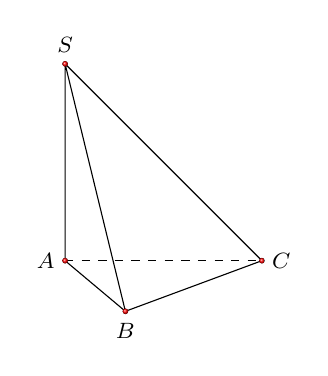
\begin{tikzpicture}[declare function={r=2.5; gocB=-40;}]
		 \path (0,0) coordinate (A)
			(90:r)  coordinate (S)
			(0:r)  coordinate (C)
			(gocB:0.4*r)  coordinate (B);
		 \draw (S)--(A)--(B)--(C)--(S)--(B);
		\draw[dashed] (A)--(C); 
		\foreach \t/\g in  {A/180,B/-90,C/0,S/90}{
			\fill[ball  color=red] (\t) circle (1pt) node[shift={(\g:7pt)},font=\footnotesize]{$ \t $};
		 }
	\end{tikzpicture}
		} 
	 \loigiai{
	\immini{Gọi $M$ là  trung điểm $BC$ thì $AM\perp BC$ và $SA\perp BC$ nên $BC\perp (SAM)$.\\
		Từ đây dễ thấy góc cần  tìm là $\alpha =\widehat{ASM}=45^\circ$.\\
		Do đó $\triangle SAM$ vuông cân ở $A$  và $SA=AM=\dfrac{a\sqrt{3}}{2}$.\\
		Suy ra $V_{S.ABC}=\dfrac{1}{3}\cdot \dfrac{a\sqrt{3}}{2}\cdot \dfrac{a^2\sqrt{3}}{4}=\dfrac{a^3}{8}$. 
		}{	\begin{tikzpicture}[declare function={r=2.5; gocB=-40;}]
		\path  (0,0) coordinate (A)
			 (90:r) coordinate (S)
			(0:r) coordinate  (C)
			(gocB:0.4*r) coordinate  (B)
			($(B)!0.5!(C)$)  coordinate (M);
		\foreach  \x/\y/\z in {A/M/B,S/M/C}{
			\path pic[draw,angle radius=5pt]{right angle=  \x--\y--\z};
		} 
		\draw (M)--(S)--(A)--(B)--(C)--(S)--(B); 
		\draw[dashed] (M)--(A)--(C); 
		\foreach  \t/\g in {A/180,B/-90,C/0,S/90,M/-60}{
			\fill[ball color=red] (\t) circle (1pt) node[shift={(\g:7pt)},font=\footnotesize]{$ \t  $};
		} 
	\end{tikzpicture}
		} 
	} 
\end{ex}

% nguồn: Ok_TracNghiemLop11_Lan1
\begin{ex}%[1H8H7-2]%[ma:0ae7cdd0]
	 Cho hình chóp $S.ABC$ có đáy là tam giác đều cạnh $a$. Biết $SA=2a$ và vuông góc với mặt phẳng $(ABC)$. Thể tích của khối chóp $S.ABC$ bằng
	\choice 
		{$a^3$} 
		{$a^3\sqrt{3}$} 
		 {$\dfrac{a^3\sqrt{3}}{2}$}
		{\True  $\dfrac{a^3\sqrt{3}}{6}$}
	 \loigiai{
		Thể tích của khối chóp  $S.ABC$ là $V=\dfrac{1}{3}Sh=\dfrac{1}{3}.\dfrac{a^2\sqrt{3}}{4}.2a=\dfrac{a^3\sqrt{3}}{6}$.
	} 
\end{ex}

% nguồn: Ok_TracNghiemLop11_Lan1
\begin{ex}%[1H8H7-2]%[ma:0a44cd02]
	Cho hình chóp $S.ABC$ có đáy $ABC$ là tam giác đều cạnh $a$. Biết $SA\perp (ABC)$ và $SA=a\sqrt{3}$. Tính thể tích khối  chóp $S.ABC$.
	\choice 
		{$\dfrac{a}{4}$} 
		 {$\dfrac{a^3}{2}$}
		{\True $\dfrac{a^3}{4}$} 
		 {$\dfrac{3a^3}{4}$}
	\loigiai{ 
	\immini 
		{ 
		$V=\dfrac{1}{3}S\cdot h=\dfrac{1}{3}\cdot  \dfrac{a^2\sqrt{3}}{4}\cdot a\sqrt{3}=\dfrac{a^3}{4}$.
		}{ 
		\begin{tikzpicture}[scale=0.5,font=\footnotesize,line join=round,line cap=round,>=stealth]
				 \path
					(0,0)  coordinate (A)
					++(-60:3) coordinate (B) 
					(5,0)  coordinate (C)
					 ($(A)+(0,4)$) coordinate (S);
				 \foreach \i in {A,B,C}{\draw (S)--(\i);}
				 \draw (A)--(B)--(C);
				 \draw[dashed](A)--(C);
				\pic[draw,angle radius=2mm] {right angle  = S--A--C};
				\foreach \i/\g in  {S/90,A/180,B/-90,C/0}
				\fill[black] (\i) circle  (1pt)+(\g:4mm) node[scale=1]{$\i$};
			\end{tikzpicture}
		 }
	} 
\end{ex}

% nguồn: Ok_Toan11_TracNghiem_Lan2
\begin{ex}%[1H8V7-2]%[ma:0e792348]
	Cho khối chóp $S.ABC$  có đáy $ABC$ là tam giác vuông tại $B$, $AB=a$, $AC=2a$, $SA \perp (ABC)$ và $SA=a$. Thể tích của khối chóp đã cho bằng
	\choice 
		 {$\dfrac{a^3\sqrt{3}}{3}$}
		 {\True $\dfrac{a^3\sqrt{3}}{6}$}
		 {$\dfrac{a^3}{3}$}
		{$\dfrac{2a^3}{3}$} 
	\loigiai{ 
		\begin{center}
			\begin{tikzpicture}[scale=1,font=\footnotesize,line join=round,line cap=round,>=stealth]
					\coordinate[label=left:$A$] (A) at (0,0); 
					\coordinate[label=right:$C$] (C)  at (3,0);
					\coordinate[label=below left:$B$] (B) at  (-40:2);
					\coordinate[label=above:$S$]  (S) at (90:3);
					\draw  (A)--(B)--(C)--(S)--cycle (S)--(B);
					\draw[dashed] (A)--(C); 
					 \foreach \diem in {A,B,C,S} \fill (\diem) circle (1pt);
					\draw  pic[draw,angle radius=0.3cm]{right angle=C--A--S};
				\end{tikzpicture}
		\end{center}
		Chiều cao  của khối chóp là $h=SA=a$.\\
		Xét tam giác đáy $ABC$  vuông tại $B$, theo định lý Pitago ta có
		$$BC = \sqrt{AC^2 - AB^2} = \sqrt{(2a)^2 -  a^2} = \sqrt{3a^2} = a\sqrt{3}.$$
		Diện tích đáy là 
		$$S_{\triangle ABC} = \dfrac{1}{2}\cdot AB \cdot BC = \dfrac{1}{2}\cdot a \cdot  a\sqrt{3} = \dfrac{a^2\sqrt{3}}{2}.$$
		Vậy thể tích  khối chóp là
		$$V = \dfrac{1}{3}\cdot S_{\triangle  ABC} \cdot SA = \dfrac{1}{3}\cdot \dfrac{a^2\sqrt{3}}{2} \cdot a = \dfrac{a^3\sqrt{3}}{6}.$$
	 }
\end{ex}

% nguồn: Ok_Toan11_TracNghiem_Lan2
\begin{ex}%[1H8V7-2]%[ma:4cc5e04b]
	Cho hình chóp $S.ABCD$ có đáy là hình chữ nhật; $AB=a$; $AD=2a$. Tam giác $SAB$ cân tại $S$ và nằm trong mặt phẳng vuông góc với đáy. Góc giữa đường thẳng $SC$ và  mp$\left(ABCD\right)$ bằng $45^{\circ}$. Gọi $M$ là trung điểm của $SD$. Tính theo $a$ khoảng cách $\mathrm{\,d}$ từ điểm $M$ đến $\left(SAC\right)$.
	\choice 
		 {\True $\mathrm{\,d}=\dfrac{a\sqrt{1513}}{89}$}
		 {$\mathrm{\,d}=\dfrac{2a\sqrt{1315}}{89}$}
		 {$\mathrm{\,d}=\dfrac{a\sqrt{1315}}{89}$}
		 {$\mathrm{\,d}=\dfrac{2a\sqrt{1513}}{89}$}
	 \loigiai{
	\immini{Gọi $H$ là trung  điểm đoạn $AB$ $\Rightarrow SH\perp\left(ABCD\right)$.\\
		Xét $\triangle  BCH$ vuông tại $B$ có $CH=\sqrt{4a^2+\dfrac{a^2}{4}}=\dfrac{a\sqrt{17}}{2}$.\\
		Xét $\triangle SHC$ vuông cân  tại $H$ có
		$SH=\dfrac{a\sqrt{17}}{2}$; $SC=\dfrac{a\sqrt{34}}{2}$.\\ 
		Xét  $\triangle SAH$ vuông tại $H$ có $SA=\sqrt{\dfrac{17a^2}{4}+\dfrac{a^2}{4}}=\dfrac{3\sqrt{2}}{2}a$.\\
		Xét $\triangle ABC$ vuông tại $B$  có $AC=\sqrt{a^2+4a^2}=a\sqrt{5}$.\\
		Suy ra ${S_{\triangle SAC}}=\dfrac{\sqrt{89}}{4}{a^2}$. 
		}{\begin{tikzpicture}[declare function={r=2; gocB=-140;}]
		 \path (0,0) coordinate (A)
			 (gocB:r) coordinate (B)
			(0:2*r) coordinate  (D)
			($(B)+(D)-(A)$)  coordinate (C)
			 ($(A)!0.5!(B)$) coordinate (H)
			($(H)+(90:1.5*r)$)  coordinate (S)
			($(S)!0.5!(D)$)  coordinate (M);
		\foreach \x/\y/\z in {S/H/B,S/H/C}{ 
			\path pic[draw,angle radius=5pt]{right angle=  \x--\y--\z};
		 }
		 \path pic["\scriptsize$45^\circ$",angle eccentricity=2,draw,fill=cyan,angle radius=12pt]{angle= S--C--H};
		\draw (S)--(B)--(C)--(D)--(S)--(C); 
		 \draw [dashed] (S)--(H)--(C)--(A)--(S)
			(B)--(A)--(D); 
		\foreach  \t/\g in {S/90,A/160,B/180,C/-60,D/0,H/-90,M/40}{
			\fill (\t) circle (1pt) node[shift={(\g:7pt)},font=\footnotesize]{$ \t $}; 
		 }
	\end{tikzpicture}
		 }\noindent
		Ta có $V_{S.ABCD}=V=\dfrac{1}{3}\cdot SH\cdot S_{ABCD}=\dfrac{a^3\sqrt{17}}{3}$, 
		 $V_{S. ACD}=\dfrac{1}{2}\cdot V=\dfrac{a^3\sqrt{17}}{6}\cdot$\\
		$V_{S.  ACM}=\dfrac{1}{2}\cdot {V_{S. ACD}}=\dfrac{a^3\sqrt{17}}{12}$.\\
		Mà  $V_{S.MAC}=\dfrac{1}{3}\cdot \mathrm{\,d}_{(M,(SAC))}\cdot S_{\triangle SAC}=\dfrac{\sqrt{89}}{12}{a^2}\cdot \mathrm{\,d}_{(M,(SAC))}$
		$\Rightarrow\mathrm{\,d}_{(M,(SAC))}=\dfrac{a\sqrt{1513}}{89}$. 
	} 
\end{ex}

% nguồn: Ok_Toan11_TracNghiem_Lan2
\begin{ex}%[1H8V7-2]%[ma:2e2ac2ba]
	Cho hình chóp $S.ABC$ có đáy $ABC$ là tam giác vuông tại $A$. Hình chiếu của $S$ lên mặt phẳng $\left(ABC\right)$ là trung điểm $H$  của $BC$, $AB=a$, $AC=a\sqrt{3}$, $SB=a\sqrt{2}$. Thể tích của khối chóp $S.ABC$ bằng
	 \choice
		{$\dfrac{a^3\sqrt{3}}{2}$} 
		{$\dfrac{a^3\sqrt{6}}{2}$} 
		 {\True $\dfrac{a^3\sqrt{3}}{6}$}
		{$\dfrac{a^3\sqrt{6}}{6}$} 
	\loigiai{ 
	\immini{Xét tam giác  $ABC$ vuông tại $A$ có\\
		$BC=\sqrt{A{B^2}+A{C^2}}=\sqrt{a^2+\left(a\sqrt{3}\right)^2}=2a$.\\ 
		$H$ là trung điểm  của $BC$ nên $BH=a$.\\
		Xét tam giác $SBH$  vuông tại $H$ có\\
		$SH=\sqrt{S{B^2}-H{B^2}}=\sqrt{\left(a\sqrt{2}\right)^2-a^2}=a$.\\ 
		Diện  tích đáy $ABC$ là $S_{ABC}=\dfrac{1}{2}AB\cdot AC=\dfrac{1}{2}{a^2}\sqrt{3}\cdot$\\
		Thể tích của  khối chóp $S.ABC$ là\\
		$V=\dfrac{1}{3}SH\cdot S_{ABC}=\dfrac{1}{3}\cdot  a\cdot \dfrac{1}{2}\cdot a^2\sqrt{3}=\dfrac{a^3\sqrt{3}}{6}$.
		}{	\begin{tikzpicture}[declare function={goc=-35; a=5; b=0.45*a; h=4;}]
		 \path
			(0,0) coordinate  (C)
			(a,0)  coordinate (A)
			(goc:b)  coordinate (B)
			($(B)!.66!(C)$) coordinate (H)--+(0,h) coordinate (S); 
		 \draw
			pic[angle radius=6pt,draw] {right angle =  S--B--A}
			pic[angle radius=6pt,draw] {right angle =  S--H--B}
			pic[angle radius=6pt,draw] {right angle = S--C--A} 
			pic[angle radius=6pt,draw] {right angle  = C--A--B};
		\draw[dashed] (A)--(C); 
		\draw (S)--(B) 
			 (S)--(H)
			(S)--(C)--(B)--(A)--cycle; 
		\foreach  \x/\goc in {S/90,C/240,A/-60,B/-90,H/-90}
		\draw[fill=white]  (\x) node[shift={(\goc:7pt)},font=\footnotesize]{$\x$} circle (1pt);
	\end{tikzpicture}
		} 
	 }
\end{ex}

% nguồn: Ok_Toan11_TracNghiem_Lan2
\begin{ex}%[1H8V7-2]%[ma:1df0a23f]
	Cho hình chóp $S.ABC$ có đáy $ABC$ là tam giác vuông cân tại $B$ và $AB=2a$. Tam giác $SAB$ đều  và nằm trong mặt phẳng vuông góc với đáy. Tính thể tích $V$ của khối chóp $S.ABC$.
	 \choice
		{$V=\dfrac{a^3\sqrt{3}}{4}$} 
		 {$V=\dfrac{a^3\sqrt{3}}{3}$}
		 {$V=\dfrac{a^3\sqrt{3}}{12}$}
		{\True $V=\dfrac{2a^3\sqrt{3}}{3}$} 
	 \loigiai{
		\begin{center}
			\begin{tikzpicture}[scale=1,font=\footnotesize,line join=round,line cap=round,>=stealth]
					\coordinate[label=left:$A$] (A)  at (0,0);
					\coordinate[label=right:$C$] (C)  at (4,0);
					\coordinate[label=below left:$B$] (B) at (-50:3); 
					 \coordinate[label=below left:$H$] (H) at ($(A)!.5!(B)$);
					\coordinate[label=above left:$S$] (S) at ($(H)+(90:4)$); 
					\draw (A)--(B)--(C)--(S)--cycle  (H)--(S)--(B);
					\draw[dashed]  (A)--(C)--(H);
					\foreach \diem  in {A,B,C,S,H} \fill (\diem) circle (1pt);
					 \draw pic[draw,angle radius=0.3cm]{right angle=S--H--B};
				\end{tikzpicture}
		\end{center}
		Gọi $H$ là trung điểm của $AB$.\\ Vì tam giác  $SAB$ đều nên $SH \perp AB$.\\
		Suy ra $SH  \perp (ABC)$.\\
		Vậy $SH$ là chiều cao  của khối chóp.\\
		Tam giác $SAB$ đều có cạnh $AB=2a$.\\ 
		Suy ra 
		$$SH = \dfrac{AB\sqrt{3}}{2} = \dfrac{2a\sqrt{3}}{2}  = a\sqrt{3}.$$
		Đáy $ABC$ là tam giác vuông cân  tại $B$ nên $BC = AB = 2a$.\\
		Khi đó, ta  có
		$$S_{\triangle ABC} = \dfrac{1}{2}\cdot AB\cdot BC = \dfrac{1}{2}\cdot 2a\cdot  2a = 2a^2.$$
		Vậy thể tích của  khối chóp là
		 $$V = \dfrac{1}{3}S_{\triangle ABC} \cdot SH = \dfrac{1}{3}\cdot 2a^2\cdot a\sqrt{3} = \dfrac{2a^3\sqrt{3}}{3}.$$
	} 
\end{ex}

% nguồn: Ok_Toan11_TracNghiem_Lan2
\begin{ex}%[1H8V7-2]%[ma:858256b1]
	Cho hình chóp $S.ABC$  có đáy $ABC$ là tam giác vuông tại $A$ và có $AB=a$, $BC=2a$.
	Mặt bên $(SAB)$  là tam giác đều và nằm trong mặt phẳng vuông góc với mặt phẳng $(ABC)$.
	Tính theo $a$ thể tích  của khối chóp $S.ABC$.
	\choice 
		 {$\dfrac{a^3}{12}$}
		{\True $\dfrac{a^3}{4}$} 
		{$\dfrac{a^3}{8}$} 
		 {$\dfrac{a^3}{6}$}
	 \loigiai{
		\begin{center}
			\begin{tikzpicture}[scale=1,font=\footnotesize,line join=round,line cap=round,>=stealth]
					\coordinate[label=left:$A$] (A) at  (0,0);
					 \coordinate[label=right:$B$] (B) at (4,0);
					\coordinate[label=below  left:$C$] (C) at (-70:2);
					 \coordinate[label=below left:$H$] (H) at ($(A)!.5!(B)$);
					\coordinate[label=above:$S$]  (S) at ($(H)+(90:3)$);
					\draw (A)--(C)--(B)--(S)--cycle  (S)--(C);
					\draw[dashed]  (A)--(B)
						(S)--(H); 
					\foreach \diem in {A,C,B,S,H} \fill (\diem)  circle (1pt);
					\draw pic[draw,angle radius=0.2cm]{right angle=B--H--S}; 
					\draw pic[draw,angle radius=0.2cm]{right angle=C--A--B}; 
					\path (A)--(H)  node[midway,sloped,scale=0.8]{$|$};
					\path  (H)--(B) node[midway,sloped,scale=0.8]{$|$};
				\end{tikzpicture}
		\end{center}
		Xét tam giác  $ABC$ vuông tại $A$, ta có
		$$ 
		AC=\sqrt{BC^2-AB^2}=\sqrt{\left(2a\right)^2-a^2}=a\sqrt{3}. 
		$$ 
		Diện tích tam giác $ABC$  là
		 $$
		S_{ABC}=\dfrac{1}{2}AB\cdot AC=\dfrac{1}{2}\cdot a\cdot  a\sqrt{3}
		 =\dfrac{a^2\sqrt{3}}{2}.
		 $$
		Gọi $H$ là trung điểm  đoạn $AB$ thì $SH\perp AB$.\\
		 Vì $(SAB)\perp (ABC)$ và $(SAB)\cap (ABC)=AB$ nên $SH\perp (ABC)$.\\
		Suy ra $SH$ là chiều cao của  khối chóp $S.ABC$.\\
		Xét  tam giác $SAH$ vuông tại $H$, ta có
		 $$
		SH = SA\cdot \sin\widehat{SAH}=a\cdot  \sin 60^\circ=\dfrac{a\sqrt{3}}{2}.
		$$ 
		Thể tích khối  chóp là
		$$ 
		V_{S.ABC}=\dfrac{1}{3}\cdot  S_{ABC}\cdot SH
		=\dfrac{1}{3}\cdot \dfrac{a^2\sqrt{3}}{2}\cdot \dfrac{a\sqrt{3}}{2} 
		 =\dfrac{a^3}{4}.
		 $$
	 }
\end{ex}

% nguồn: Ok_Toan11_TracNghiem_Lan2
\begin{ex}%[1H8V7-2]%[ma:edb25e9a]
	Cho hình chóp $S.ABC$ có đáy $ABC$ là tam giác đều, $SA\perp(ABC)$. Mặt phẳng $(SBC)$ cách  $A$ một khoảng bằng $a$ và hợp với mặt phẳng $(ABC)$ góc $30^\circ$. Thể tích của khối chóp $S.ABC$ bằng
	\choice 
		{\True  $\dfrac{8a^3}{9}$}
		 {$\dfrac{8a^3}{3}$}
		{$\dfrac{\sqrt{3}a^3}{12}$} 
		 {$\dfrac{4a^3}{9}$}
	\loigiai{ 
	\immini 
		{ 
		Gọi  $I$ là trung điểm sủa $BC$ suy ra góc giữa $(SBC)$ và $(ABC)$ là $\widehat{SIA}=30^\circ$.\\
		Gọi $H$ là hình chiếu vuông góc của $A$ trên  $SI$ suy ra\\ $\mathrm{d}(A,(SBC))=AH=a$.\\
		 Xét tam giác $AHI$ vuông tại $H$ suy ra $AI=\dfrac{AH}{\sin{30^\circ}}=2a$.\\
		Giả  sử tam giác đều $ABC$ có cạnh bằng $x$, mà $AI$ là đường cao suy ra $2a=x\dfrac{\sqrt{3}}{2}\Rightarrow x=\dfrac{4a}{\sqrt{3}}$.\\
		Diện tích tam  giác đều $ABC$ là $S_{ABC}=\left(\dfrac{4a}{\sqrt{3}}\right)^2\cdot \dfrac{\sqrt{3}}{4}=\dfrac{4a^2\sqrt{3}}{3}$.\\
		Xét tam giác $SAI$ vuông tại $A$  suy ra $SA=AI\cdot \tan{30^\circ}=\dfrac{2a}{\sqrt{3}}$.\\
		Vậy $V_{S.ABC}=\dfrac{1}{3}\cdot S_{ABC}\cdot SA=\dfrac{1}{3}\cdot \dfrac{4a^2\sqrt{3}}{3}\cdot  \dfrac{2a}{\sqrt{3}}=\dfrac{8a^3}{9}$.
		} 
		 {
		\begin{tikzpicture}[>=stealth,line join=round,line cap=round,font=\footnotesize,scale=1]
				\def\a{4} 
				 \def\b{3}
				 \def\h{3}
				\path 
					 (0,0) coordinate (A)
					+(90:\h) coordinate  (S)
					+ (0:\a) coordinate  (C)
					 + (-30:\b) coordinate (B)
					($(B)!.5!(C)$) coordinate  (I)
					($(S)!.4!(I)$)  coordinate (H);
				 \draw (S)--(A)--(B)--(C)--cycle (S)--(B)
					(S)--(I); 
				\draw[dashed] (A)--(C) 
					(A)--(I) 
					 (A)--(H);
				\foreach \x/\g in {S/90,A/180,B/-90,C/0,I/-30,H/10} \fill (\x) circle (0.03)+(\g:3mm) node[scale=.9]  {$\x$};
			\end{tikzpicture}
		 }
	 }
\end{ex}

% nguồn: Ok_Toan11_TracNghiem_Lan2
\begin{ex}%[1H8V7-2]%[ma:4482827d]
	Cho hình chóp $S.ABC$ có đáy $ABC$ là tam giác vuông tại $A$  và có $AB=a$, $BC=a\sqrt{3}$.
	Mặt bên $(SAB)$ là tam giác đều và nằm trong mặt phẳng vuông  góc với mặt phẳng $(ABC)$.
	Tính theo  $a$ thể tích của khối chóp $S.ABC$.
	\choice 
		{$\dfrac{a^3\sqrt{6}}{6}$} 
		 {\True $\dfrac{a^3\sqrt{6}}{12}$}
		 {$\dfrac{2a^3\sqrt{6}}{3}$}
		 {$\dfrac{a^3\sqrt{6}}{4}$}
	 \loigiai{
		\begin{center}
			\begin{tikzpicture}[scale=1,font=\footnotesize,line join=round,line cap=round,>=stealth]
					\coordinate[label=left:$A$]  (A) at (0,0);
					\coordinate[label=right:$B$] (B) at (4,0); 
					\coordinate[label=below left:$C$] (C) at  (-70:2);
					\coordinate[label=below left:$H$] (H)  at ($(A)!.5!(B)$);
					\coordinate[label=above:$S$] (S)  at ($(H)+(90:3)$);
					 \draw (A)--(C)--(B)--(S)--cycle (S)--(C);
					 \draw[dashed] (A)--(B)
						(S)--(H); 
					\foreach \diem in {A,C,B,S,H} \fill (\diem)  circle (1pt);
					\draw pic[draw,angle radius=0.2cm]{right angle=B--H--S}; 
					\draw pic[draw,angle radius=0.2cm]{right  angle=C--A--B};
					\path (A)--(H) node[midway,sloped,scale=0.8]{$|$}; 
					\path (H)--(B)  node[midway,sloped,scale=0.8]{$|$};
				\end{tikzpicture}
		\end{center}
		Gọi $H$ là trung điểm của  cạnh $AB$. \\
		Do $\triangle SAB$ đều nên $SH \perp  AB$.\\
		Ta có 
		$\heva{ 
		&(SAB)\perp (ABC)\\  &(SAB)\cap(ABC)=AB\\
		&SH\subset  (SAB), SH\perp AB.
		 }$\\
		Suy ra $SH \perp  (ABC)$.\\
		 Suy ra $SH$ là chiều cao của khối chóp $S.ABC$.\\
		Xét $\triangle ABC$ vuông tại $A$, ta  có
		 $$
		 AC=\sqrt{BC^2-AB^2}=\sqrt{\left(a\sqrt{3}\right)^2-a^2}=a\sqrt{2}.
		$$ 
		Diện  tích đáy là
		$$ 
		 S_{ABC}=\dfrac{1}{2}AB\cdot AC=\dfrac{1}{2}\cdot a\cdot a\sqrt{2}=\dfrac{a^2\sqrt{2}}{2}.
		$$ 
		Mặt khác,  ta có $\triangle SAB$ đều cạnh $a$, nên chiều cao $SH=\dfrac{a\sqrt{3}}{2}$.\\
		Do  đó thể tích khối chóp là
		$$ 
		V_{S.ABC}=\dfrac{1}{3}\cdot S_{ABC}\cdot  SH
		=\dfrac{1}{3}\cdot \dfrac{a^2\sqrt{2}}{2}\cdot \dfrac{a\sqrt{3}}{2} 
		 =\dfrac{a^3\sqrt{6}}{12}.
		$$ 
	} 
\end{ex}

% nguồn: Ok_Toan11_TracNghiem_Lan2
\begin{ex}%[1H8V7-2]%[ma:fa9613fc]
	Cho hình chóp $S.ABC$ có đáy $ABC$  là tam giác đều cạnh $a$.
	Hình chiếu vuông góc của $S$ trên  đáy là điểm $H$ trên cạnh $AC$ sao cho $AH=\dfrac{2}{3}AC$. Mặt phẳng $(SBC)$ tạo với đáy một góc $60^\circ$.
	 Thể tích khối chóp $S.ABC$ là
	\choice 
		{$\dfrac{a^3\sqrt{3}}{12}$} 
		{\True $\dfrac{a^3\sqrt{3}}{48}$} 
		{$\dfrac{a^3\sqrt{3}}{36}$} 
		{$\dfrac{a^3\sqrt{3}}{24}$} 
	 \loigiai{
		\begin{center}
			\begin{tikzpicture}[scale=1,font=\footnotesize,line join=round,line cap=round,>=stealth]
					\coordinate[label=left:$A$] (A) at  (0,0);
					\coordinate[label=right:$B$] (B)  at (5,0);
					\coordinate[label=below left:$C$]  (C) at (-25:4);
					 \coordinate[label=above:$S$] (S) at (60:4);
					\coordinate[label=right:$M$]  (M) at ($(B)!0.5!(C)$);
					\coordinate[label=below:$H$]  (H) at ($(A)!0.4!(C)$);
					 \coordinate[label=right:$N$] (N) at ($(C)!0.25!(B)$);
					\draw (A)--(C)--(B)--(S)--cycle (H)--(S)--(C) 
						 (S)--(N);
					\draw[dashed]  (M)--(A)--(B)
						 (H)--(N);
					\foreach \diem in {A,C,B,S,M,H,N}  \fill (\diem) circle (1pt);
					\draw pic[draw,angle radius=0.2cm]{right  angle=S--H--A};
				\end{tikzpicture}
		\end{center}
		Gọi $M$ là trung  điểm của $BC$.\\
		Lấy $N\in CM$ sao  cho $\dfrac{CN}{CM}=\dfrac{CH}{CA}=\dfrac{1}{3}$.\\
		Suy ra $HN\parallel  AM$.\\
		Vì $\triangle ABC$ đều nên $AM\perp  BC$. Khi đó $HN\perp BC$.\\
		Suy ra  $BC\perp (SHN)$.\\
		Khi đó $\left(\widehat{(SBC),(ABC)}\right)=\widehat{HNS}=60^\circ$.\\ 
		Do $\triangle ABC$ đều nên $AM=\dfrac{a\sqrt{3}}{2}$. Suy  ra $HN=\dfrac{1}{3}AM=\dfrac{a\sqrt{3}}{6}$.\\
		Xét  $\triangle SHN$ vuông tại $H$, ta có
		 $$
		SH = HN\cdot \sin\widehat{SNH} 
		 = \dfrac{a\sqrt{3}}{6}\cdot \sin 60^\circ = \dfrac{a}{4}.
		$$ 
		Diện tích đáy $S_{ABC}=\dfrac{a^2\sqrt{3}}{4}$.\\ 
		Thể tích  hình chóp là
		 $$
		V_{S.ABC}=\dfrac{1}{3}\cdot SH\cdot  S_{ABC}
		= \dfrac{1}{3}\cdot \dfrac{a}{4}\cdot \dfrac{a^2\sqrt{3}}{4} 
		 = \dfrac{a^3\sqrt{3}}{48}.
		 $$
	 }
\end{ex}

% nguồn: Ok_Toan11_TracNghiem_Lan2
\begin{ex}%[1H8V7-2]%[ma:3c43688a]
	Cho  hình chóp $S.ABC$ có $AB=a$, $BC=a\sqrt{3}$, $\widehat{ABC}=60^\circ$.
	Hình chiếu vuông góc của $S$  lên mặt phẳng $(ABC)$ là một điểm thuộc cạnh $BC$.
	Góc giữa đường thẳng $SA$ và mặt phẳng $(ABC)$ là  $45^\circ$.
	 Giá trị nhỏ nhất của thể tích khối chóp $S.ABC$ bằng
	\choice 
		{$\dfrac{a^3\sqrt{3}}{3}$} 
		{\True  $\dfrac{a^3\sqrt{3}}{8}$}
		{$\dfrac{a^3\sqrt{3}}{12}$} 
		 {$\dfrac{a^3\sqrt{3}}{6}$}
	 \loigiai{
		\begin{center}
			\begin{tikzpicture}[scale=1,font=\footnotesize,line join=round,line cap=round,>=stealth]
					\coordinate[label=left:$B$] (B)  at (0,0);
					\coordinate[label=right:$A$]  (A) at (4,0);
					\coordinate[label=below  left:$C$] (C) at (-45:3);
					\coordinate[label=below left:$H$] (H) at ($(B)!.5!(C)$); 
					\coordinate[label=above left:$S$] (S)  at ($(H)+(90:4)$);
					\draw  (B)--(C)--(A)--(S)--cycle (H)--(S)--(C);
					\draw[dashed] (B)--(A)--(H); 
					\foreach \diem in {B,C,A,S,H}  \fill (\diem) circle (1pt);
					\draw pic["$45^\circ$",draw,angle  eccentricity=1.5,angle radius=0.5cm]{angle=S--A--H};
					\draw pic["$60^\circ$",draw,angle eccentricity=1.65,angle radius=0.5cm]{angle=C--B--A}; 
					\draw  pic[draw,angle radius=0.3cm]{right angle=C--H--S};
				\end{tikzpicture}
		\end{center}
		Gọi $H$ là hình chiếu của $S$ lên mặt phẳng  $(ABC)$, khi đó $H \in BC$.\\
		Ta có $\widehat{(SA,(ABC))} = \widehat{SAH} = 45^\circ$. Suy ra $\triangle SHA$  vuông cân.\\
		Suy ra  $SH = HA$.\\
		Khi  đó, ta có
		 \allowdisplaybreaks
		\begin{eqnarray*}
			 V_{S.ABC} &=& \dfrac{1}{3}\cdot S_{ABC}\cdot SH\\
			&=& \dfrac{1}{3}\cdot \dfrac{1}{2}AB\cdot BC \cdot \sin \widehat{ABC}\cdot  SH\\
			&=& \dfrac{1}{6}\cdot  a \cdot a\sqrt{3}\cdot \sin 60^\circ \cdot AH\\
			&=& \dfrac{a^2}{4}\cdot  AH.
		\end{eqnarray*}
		Thể tích nhỏ nhất khi $AH$ nhỏ nhất. Khi đó $AH \perp BC$ tại $H$.\\ 
		Xét tam  giác $ABH$, ta có
		 $$
		\sin \widehat{ABH}  = \dfrac{AH}{AB} \Rightarrow AH = a\sin 60^\circ = \dfrac{a\sqrt{3}}{2}.
		$$ 
		Vậy 
		 $$
		 V_{\min} = \dfrac{a^2}{4}\cdot \dfrac{a\sqrt{3}}{2}
		= \dfrac{a^3\sqrt{3}}{8}. 
		 $$
	} 
\end{ex}

% nguồn: Ok_Toan11_TracNghiem_Lan2
\begin{ex}%[1H8V7-2]%[ma:61f80a1f]
	Cho hình chóp tam giác đều  $S.ABC$ có độ dài cạnh đáy bằng $a$, góc hợp bởi cạnh bên và mặt đáy bằng $60^{^\circ}$. Thể tích của khối chóp đã cho bằng
	 \choice
		 {\True $\dfrac{a^3\sqrt{3}}{12}$}
		{$\dfrac{a^3\sqrt{3}}{3}$} 
		{$\dfrac{a^3\sqrt{3}}{6}$} 
		{$\dfrac{a^3\sqrt{3}}{4}$} 
	 \loigiai{
	\immini{ 
		Gọi $H$ là trọng tâm của tam  giác đều $ABC$.\\
		Khi đó $SH\perp (ABC)$,  $AH=\dfrac{AB\sqrt{3}}{3}=\dfrac{a\sqrt{3}}{3}$.\\
		Theo đề bài ta có $\widehat{\left(SA,(ABC)\right)}=\widehat{SAH}=60^\circ$.\\ 
		Xét $\Delta SAH$ vuông tại $H$, có $SH=AH\cdot \tan 60^\circ  =\dfrac{a\sqrt{3}}{3}\cdot \sqrt{3}=a$.\\
		Thể tích  $V_{S.ABC}=\dfrac{1}{3}SH\cdot{S_{\Delta ABC}}=\dfrac{1}{3}a\cdot \dfrac{a^2\sqrt{3}}{4}=\dfrac{a^3\sqrt{3}}{12}$.
		 }{
		\begin{tikzpicture}[scale=1,>=stealth,line join=round,line cap=round,font=\footnotesize]
				\def\a{4} 
				\def\h{3.5} 
				 \def\r{1.5}
				\def\al{-40} 
				 \path
					(0,0) coordinate  (A)
					(\al:\r)  coordinate (B)
					(\a,0) coordinate  (C)
					 ($(B)!1/2!(C)$) coordinate (M)
					($(A)!2/3!(M)$) coordinate (O) 
					($(O)$) coordinate (H) 
					($(O)+(0,\h)$) coordinate (S); 
				\draw (S)--(A)--(B)--(S)--(C)--(B) 
					 (S)--(M);
				 \draw[dashed,thin] (A)--(C)
					(S)--(O) 
					(A)--(M); 
				\foreach \p/\g in {A/160,B/-120,C/0,S/90,H/-120,M/-45}\fill (\p)  circle (1pt) node[shift={(\g:.3)}]{$\p$};
				\foreach \a/\b/\c in {S/H/A} 
					{\draw pic[draw,angle radius=2mm]  {right angle = \a--\b--\c};};
			\end{tikzpicture}
		} 
	} 
\end{ex}

% nguồn: Ok_Toan11_TracNghiem_Lan2
\begin{ex}%[1H8V7-2]%[ma:6640d687]
	Cho hình chóp $S.ABC$ có đáy là tam giác cân tại $A$, $AB=AC=a$,  $\widehat{BAC}=120^\circ$.
	Tam giác $SAB$ là tam giác  đều và nằm trong mặt phẳng vuông góc với mặt đáy.
	Tính thể tích  $V$ của khối chóp $S.ABC$.
	 \choice
		 {\True $\dfrac{a^3}{8}$}
		{$a^3$} 
		 {$\dfrac{a^3}{2}$}
		{$2a^3$} 
	 \loigiai{
		\begin{center}
			\begin{tikzpicture}[scale=1,font=\footnotesize,line join=round,line cap=round,>=stealth]
					\coordinate[label=left:$A$]  (A) at (0,0);
					\coordinate[label=right:$C$] (C) at  (4,0);
					 \coordinate[label=below left:$B$] (B) at (-50:3);
					\coordinate[label=below left:$H$] (H) at  ($(A)!.5!(B)$);
					\coordinate[label=above left:$S$] (S) at ($(H)+(90:4)$); 
					\draw (A)--(B)--(C)--(S)--cycle (H)--(S)--(B); 
					 \draw[dashed] (A)--(C)--(H);
					\foreach \diem in {A,B,C,S,H}  \fill (\diem) circle (1pt);
					 \draw pic[draw,angle radius=0.2cm]{right angle=C--H--S};
					 \draw pic[draw,angle radius=0.2cm]{right angle=S--H--A};
				\end{tikzpicture}
		\end{center}
		Gọi $H$ là trung điểm của $AB$.\\ 
		Vì tam giác $SAB$ đều nên $SH  \perp AB$.\\
		Ta có 
		$\heva{ 
		 &(SAB)\perp (ABC)\\ &(SAB)\cap(ABC)=AB\\
		&SH\subset (SAB), SH\perp  AB.
		}$\\ 
		Suy ra $SH$ là chiều  cao của hình chóp $S.ABC$.\\
		Nhận thấy $\triangle SAB$ là tam giác đều cạnh $a$ nên  $
		 SH=\dfrac{a\sqrt{3}}{2}$.\\
		Diện tích tam  giác $ABC$ là
		$$ 
		S_{ABC}=\dfrac{1}{2}\cdot AB\cdot  AC\cdot \sin 120^\circ
		 =\dfrac{1}{2}\cdot a\cdot a\cdot \dfrac{\sqrt{3}}{2}
		=\dfrac{a^2\sqrt{3}}{4}. 
		 $$
		Thể  tích khối chóp là
		 $$
		V_{S.ABC}=\dfrac{1}{3}\cdot SH\cdot  S_{ABC}
		=\dfrac{1}{3}\cdot \dfrac{a\sqrt{3}}{2}\cdot  \dfrac{a^2\sqrt{3}}{4}
		 =\dfrac{a^3}{8}.
		 $$
	 }
\end{ex}

% nguồn: Ok_Toan11_TracNghiem_Lan2
\begin{ex}%[1H8C7-2]%[ma:af009401]
	Cho hình  chóp đều $S.ABC$ có $SA=a$. Gọi $D$, $E$ lần lượt là trung điểm của $SA$, $SC$. Tính thể tích khối chóp $S.ABC$ theo $a$, biết $BD \perp AE$.
	 \choice
		 {\True $\dfrac{a^3\sqrt{21}}{54}$}
		{$\dfrac{a^3\sqrt{3}}{12}$} 
		{$\dfrac{a^3\sqrt{7}}{27}$} 
		 {$\dfrac{a^3\sqrt{21}}{27}$}
	\loigiai{ 
		\begin{center}
			\begin{tikzpicture}[scale=1,font=\footnotesize,line join=round,line cap=round,>=stealth]
					 \coordinate[label=left:$A$] (A) at (0,0);
					 \coordinate[label=right:$C$] (C) at (4,0);
					\coordinate[label=below left:$B$] (B) at  (-50:3);
					\coordinate[label=above:$S$] (S) at (70:4); 
					\coordinate[label=left:$D$] (D) at ($(S)!0.5!(A)$); 
					\coordinate[label=right:$E$] (E)  at ($(S)!0.5!(C)$);
					\coordinate[label=right:$F$] (F)  at ($(S)!0.5!(E)$);
					 \draw (A)--(B)--(C)--(S)--cycle (S)--(B)
						 (F)--(B)--(E)
						(B)--(D); 
					\draw[dashed]  (E)--(A)--(C)
						 (D)--(F);
					\foreach \diem  in {A,B,C,S,D,E,F} \fill (\diem) circle (1pt);
				\end{tikzpicture}
		\end{center}
		Gọi $F$ là  trung điểm $SE$. Suy ra $BD \perp DF$.\\
		Đặt  $AB = x$. Ta có\\
		 \allowdisplaybreaks
		\begin{eqnarray*}
			BE^2 = BD^2  = AE^2 &=& \dfrac{2AS^2 + 2AC^2 - SC^2}{2}\\
			 &=& \dfrac{2a^2 + 2x^2 - a^2}{2}\\
			&=&  \dfrac{a^2 + 2x^2}{2}.
		\end{eqnarray*}
		Suy ra 
		\allowdisplaybreaks 
		\begin{eqnarray*}
			BF^2 &=& \dfrac{2BS^2 + 2BE^2 -  SE^2}{4} \\
			&=& \dfrac{2a^2  + \dfrac{a^2+2x^2}{2} - \dfrac{a^2}{4}}{4} \\
			&=&  \dfrac{9a^2 + 4x^2}{16}.
		\end{eqnarray*}
		 Mặt khác, ta có
		 \allowdisplaybreaks
		\begin{eqnarray*}
			&&BF^2 = \dfrac{BD^2 + DF^2}{2} =  \dfrac{5BD^2}{4}\\
			&\Rightarrow& BF^2 = \dfrac{5}{4} \cdot \dfrac{a^2+2x^2}{2}= \dfrac{5a^2 +  10x^2}{8}\quad (*).
		\end{eqnarray*}
		 Khi đó, ta có
		 \allowdisplaybreaks
		\begin{eqnarray*}
			(*)&\Leftrightarrow&\dfrac{9a^2+4x^2}{16}  = \dfrac{5a^2+10x^2}{8}\\
			&\Leftrightarrow& 9a^2 + 4x^2  = 10a^2 + 20x^2\\
			&\Leftrightarrow& x^2  = \dfrac{2}{3}a^2.
		\end{eqnarray*}
		Do đó  $x = a\sqrt{\dfrac{2}{3}}$.\\
		Gọi $H$ là  hình chiếu của $S$ lên $(ABC)$, khi đó $H$ là tâm đường tròn ngoại tiếp $\triangle ABC$.\\
		Khi đó, ta  có
		 $$
		SH  = \sqrt{SA^2 - AH^2}
		= \sqrt{a^2 - \left(\dfrac{2}{3}\cdot x\cdot \dfrac{\sqrt{3}}{2}\right)^2} 
		=  \dfrac{a\sqrt{7}}{3}.
		 $$
		Tam  giác $ABC$ đều cạnh $x$ nên
		 $$
		S_{ABC} =  \dfrac{x^2\sqrt{3}}{4} = \dfrac{a^2 \sqrt{3}}{6}.
		 $$
		Vậy  thể tích khối chóp là
		$$ 
		V_{S.ABC} = \dfrac{1}{3} \cdot SH \cdot  S_{ABC}
		= \dfrac{1}{3} \cdot \dfrac{a\sqrt{7}}{3} \cdot \dfrac{a^2 \sqrt{3}}{6} 
		 = \dfrac{a^3 \sqrt{21}}{54}.
		 $$
	} 
\end{ex}


%%%%%%%%%%%%%%%% ĐÚNG/SAI %%%%%%%%%%%%%%%%

% nguồn: Ok_dungsai_lop11_Lan1
\begin{ex}%[1H8H7-2]%[1H8V2-2]%[ma:a3ee206a]
 Cho tứ diện $OABC$ có các cạnh $OA$, $OB$, $OC$ đôi một vuông góc với nhau. Gọi $H$  là trực tâm của tam giác $ABC$. Xét tính đúng sai của các mệnh đề sau
 \choiceTF 
  {\True  $OA\perp (OBC)$}
  {$V_{OABC}=\dfrac{1}{3}\cdot OA\cdot OB\cdot OC$} 
   {\True $OH\perp (ABC)$}
   {\True $\dfrac{1}{OH^2}=\dfrac{1}{OA^2}+\dfrac{1}{OB^2}+\dfrac{1}{OC^2}$}
 \loigiai{ 
  \immini{
  Gọi $K$ và $L$ lần lượt là chân đường cao kẻ  từ $C$ và $B$ của tam giác $ABC$.
  \begin{itemize}
    \item $\heva{&OA\perp OB\\&OA\perp OC}\Rightarrow OA\perp (OBC)$.
   \item  $\heva{&OC\perp OB\\&OC\perp OA}\Rightarrow OC\perp (OAB) \Rightarrow OC \perp AB$.\\
   $\heva{&AB\perp SK\\& AB\perp OC}\Rightarrow AB\perp (OCK) \Rightarrow AB\perp  OH$.
  \end{itemize}
  }{ 
  \begin{tikzpicture}[font=\footnotesize,line join=round,line cap=round,>=stealth,scale=0.8]
    \foreach \x/\y/\pos in {0/0/O,-1.5/-1.7/B,4/0/C} \path ($(\x,\y)$)  coordinate (\pos);
    \path 
      ($(O)+(0,4)$) coordinate (A)
     ($(A)!.5!(B)$) coordinate  (K)
      ($(A)!.6!(C)$) coordinate (L)
     (intersection of B--L  and C--K) coordinate (H);
    \draw[dashed] (C)--(O)--(B) 
     (H)--(O)--(A); 
     \draw
     (A)--(B)--(C)--cycle 
      (B)--(L)
      (C)--(K);
    \foreach \x/\pos in {A/90,B/-150,C/-30,O/-90,H/-90,L/30,K/150} \fill  (\x) circle (1pt) node[{shift=(\pos:0.25)}]{$\x$};
   \end{tikzpicture}
  } 
   \noindent
  \begin{itemize}
   \item $\heva{&OB\perp OA\\&OB\perp OC}\Rightarrow OB\perp (OAC)  \Rightarrow OB \perp CA$.\\
   $\heva{&CA\perp BL\\& CA\perp OB}\Rightarrow CA\perp (OBL) \Rightarrow CA\perp  OH.$
   \item $\heva{&AB\perp OH \\&CA\perp OH} \Rightarrow  OH\perp (ABC)$.
  \end{itemize}
  $\triangle OAB$ vuông tại  $O$ có $OK$ là đường cao $\Rightarrow \dfrac{1}{OK^2}=\dfrac{1}{OA^2}+\dfrac{1}{OB^2}$.\\
  $\triangle OKS$ vuông  tại $O$ có $OH$ là đường cao ($OH\perp CK$ do $OH \perp (ABC)$).\\
  $\Rightarrow  \dfrac{1}{OH^2}=\dfrac{1}{OC^2}+\dfrac{1}{OK^2} \Rightarrow \dfrac{1}{OH^2}=\dfrac{1}{OA^2}+\dfrac{1}{OB^2}+\dfrac{1}{OC^2}$.
  \begin{itemchoice}
   \itemch  Ta có $OA\perp (OBC)$.
   \itemch Ta có $V_{OABC}=\dfrac{1}{3}\cdot  OA\cdot S_{OBC}=\dfrac{1}{3}\cdot OA\cdot\dfrac{1}{2}\cdot OB\cdot OC=\dfrac{1}{6}\cdot OA\cdot OB\cdot OC$.
   \itemch $OH \perp  (ABC)$.
   \itemch $\dfrac{1}{OH^2}=\dfrac{1}{OA^2}+\dfrac{1}{OB^2}+\dfrac{1}{OC^2}$. 
  \end{itemchoice}
  }
\end{ex}

% nguồn: Ok_dungsai_lop11_Lan1
\begin{ex}%[1H8V7-2]%[ma:d8c7c9ae]
 Cho hình chóp $S. A B C$ có mặt bên $(S A B)$ vuông góc với mặt đáy và tam giác $S A B$ đều cạnh $2 a$. Biết tam giác $A B C$ vuông tại $C$ và  cạnh $A C=a \sqrt{3}$. Khi đó:
  \choiceTF
   {\True $S H \perp(A B C)$}
   {\True $\mathrm{d}(S,(ABC))=a\sqrt{3}$}
   {$\mathrm{d}(C,(SAB))=\dfrac{a\sqrt{3}}{3}$}
  {Thể  tích của khối chóp $S. A B C$ bằng $\dfrac{a^3}{6}$}
 \loigiai{ 
  \begin{center}
   \begin{tikzpicture}[scale=1,font=\footnotesize,line join=round,line cap=round,>=stealth]
     \path 
      (0,0) coordinate (B) 
      ++(-45:2) coordinate (C) 
       (5,0) coordinate (A)
       ($(A)!1/2!(B)$) coordinate (H)
       ($(H)+(0,3.5)$) coordinate (S)
      ($(A)!(C)!(B)$) coordinate (K); 
      \foreach \i in {A,B,C}{\draw (S)--(\i);}
     \draw (A)--(C)--(B); 
     \draw[dashed,thin](A)--(B) 
      (S)--(H) 
       (C)--(K);
     \pic[draw,thin,angle radius=2mm]  {right angle = S--H--A};
     \pic[draw,thin,angle radius=2mm] {right angle = B--C--A}; 
      \pic[draw,thin,angle radius=2mm] {right angle = C--K--B};
     \foreach \i/\g in  {S/90,A/0,B/180,C/-90,H/-90,K/90}
     \fill[black] (\i) circle (1pt)+(\g:4mm) node[scale=1]{$\i$}; 
      \path (S)--(B) node[left,midway]{$2a$};
     \path (S)--(A) node[right,midway]{$2a$}; 
      \path (C)--(A) node[right,midway]{$a\sqrt{3}$};
     \path (B)--(A) node[above,pos=.7]{$2a$}; 
    \end{tikzpicture}
  \end{center}
  \begin{itemchoice}
   \itemch Gọi $H$ là trung điểm $A B$, mà tam giác  $S A B$ đều nên $S H \perp A B$. \\
   Ngoài ra $(S A B) \perp(A B C)$ nên $S H \perp(A B  C)$.
   \itemch Ta có $\mathrm{d}(S,(A B C))=S H=\dfrac{2 a \cdot \sqrt{3}}{2}=a \sqrt{3}$ (do tam  giác $S A B$ đều cạnh $2 a)$.
   \itemch Kẻ đường cao $C K$ của tam giác $A B C$.\\ 
   Ta có $\heva{&C K \perp A B \\ &C K \perp S H}\Rightarrow C K \perp(S A B) \Rightarrow \mathrm{d}(C,(S A B))=C K$.\\ 
   Xét tam giác $A B C$ vuông  tại $C$ có\\
   $B C=\sqrt{A B^2-A  C^2}=\sqrt{4 a^2-3 a^2}=a; C K=\dfrac{C A \cdot C B}{A B}=\dfrac{a \sqrt{3} \cdot a}{2 a}=\dfrac{a \sqrt{3}}{2}$.\\
   Vậy $\mathrm{d}(C,(S  A B))=C K=\dfrac{a \sqrt{3}}{2}$.\\
   \itemch Diện tích đáy hình chóp  là: $S_{\Delta A B C}=\dfrac{1}{2} A C \cdot B C=\dfrac{1}{2} a \sqrt{3} \cdot a=\dfrac{a^2 \sqrt{3}}{2}$.
   Thể tích khối chóp là: $\mathrm{V}_{S \cdot A B C}=\dfrac{1}{3} S H \cdot S_{\Delta A B C}=\dfrac{1}{3} \cdot a \sqrt{3} \cdot \dfrac{a^2 \sqrt{3}}{2}=\dfrac{a^3}{2}$ 
  \end{itemchoice}
  }
\end{ex}


%%%%%%%%%%%%%%%% TỰ LUẬN %%%%%%%%%%%%%%%%

% nguồn: Ok_TuanLuan_Toan11_Lan2
\begin{ex}%[1H8H7-2]%[ma:80b809b9]
	Cho khối  chóp $S.ABC$ có $SA \perp (ABC)$, $SA=a$, $AB=a$, $AC=2a$ và $\widehat{BAC}=120^{\circ}$. Tính thể tích khối chóp $S.ABC$.
	 \loigiai{
		\begin{center}
			\begin{tikzpicture}[scale=1,font=\footnotesize,line join=round,
						 line cap=round,>=stealth]
					\path (0:0) coordinate (A) 
						++(0:4)  coordinate (C)
						++(-150:3.2) coordinate (B) 
						 ($(A)+(90:3)$) coordinate (S);
					\draw[] (A)--(B)--(C) 
						 (A)--(S)
						 (B)--(S)
						(C)--(S); 
					 \draw[dashed] (A)--(C);
					\foreach  \x /\goc in {A/180,B/-135,C/0,S/90}
					\fill (\x)  circle (1pt)
						($(\x)+(\goc:3mm)$) node  {$\x$};
					 \foreach \x/\y/\z in {S/A/C}{\draw pic[draw,angle radius=2mm]{right angle=\x--\y--\z};}
				\end{tikzpicture}
		\end{center}
		Ta  có
		$$S_{\triangle ABC}=\dfrac{1}{2}\,AB \cdot AC \cdot \sin \widehat{BAC} 
		=\dfrac{1}{2}\cdot a \cdot 2a \cdot  \sin 120^{\circ}
		=\dfrac{a^2\sqrt{3}}{2}.$$ 
		 Nên
		$$V_{S.ABC}=\dfrac{1}{3}a \cdot  \dfrac{a^2\sqrt{3}}{2}
		=\dfrac{a^3\sqrt{3}}{6}~\text{(đvtt}.$$ 
	} 
\end{ex}

% nguồn: Ok_TuanLuan_Toan11_Lan2
\begin{ex}%[1H8H7-2]%[ma:d5c93416]
	Cho hình chóp $S.ABC$ có đáy $ABC$ là tam giác đều cạnh $a$. Hình chiếu của đỉnh $S$ lên mặt phẳng $(ABC)$ là điểm $H$ đối xứng với $A$ qua $BC$.  Biết $SA=2a$. Tính thể tích của khối chóp $S.ABC$ theo $a$.
	 \loigiai{
	 \immini
		 {
		Vì $H$ đối xứng với $A$ qua $BC$ và  $\triangle ABC$ đều nên\\ $AH=2\cdot\dfrac{a\sqrt{3}}{2}=a\sqrt{3}$.\\
		Do $SH\perp(ABC)$ nên tam giác $SAH$ vuông tại $H$, do đó\\ $SH=\sqrt{SA^2-AH^2}=\sqrt{4a^2-3a^2}=a$.\\ 
		Vậy thể tích  của khối chóp $S.ABC$ là $$V_{S.ABC}=\dfrac{1}{3}\cdot SH\cdot S_{\triangle ABC}=\dfrac{1}{3}\cdot a\cdot\dfrac{\sqrt{3}a^2}{4}=\dfrac{\sqrt{3}a^3}{12}.$$
		 }
		{ 
		\begin{tikzpicture}[>=stealth,line join=round,line cap=round,font=\footnotesize,scale=0.7,declare function={a=3; b=2.5;}]
				\path 
					(a,0) coordinate (C) 
					(-a,0) coordinate  (B)
					(60:b)  coordinate (H)
					($(0,0)-(H)$) coordinate (A) 
					($(H)+(90:b)$)  coordinate (S);
				 \draw (B)--(A)--(C);
				\draw (S)--(C) 
					(B)--(S)--(A); 
				\draw[dashed]  (B)--(H)--(C)--(B)
					(S)--(H)--(A); 
				\draw pic[draw,angle  radius=2mm]{right angle=S--H--B};
				\draw pic[draw,angle radius=2mm]{right  angle=C--H--S};
				\draw  pic[draw,angle radius=2mm]{right angle=B--A--C};
				\foreach \i \g in {A/-90,B/180,C/0,H/15,S/90}\fill (\i)  circle (1pt)+(\g:.4) node{$\i$};
			\end{tikzpicture}
		} 
	} 
\end{ex}

% nguồn: Ok_TuanLuan_Toan11_Lan2
\begin{ex}%[1H8H7-2]%[ma:5ec3d71e]
	Cho hình chóp $S.ABC$ có đáy $ABC$ là tam giác vuông tại $A$, $AB=a$, $AC=2a$. Cạnh bên $SA$ vuông góc với đáy và $SA=2a$. Tính thể tích $V$ của  khối chóp $S.ABC$.
	 \loigiai{
		\begin{center}
			\begin{tikzpicture}[scale=1,font=\footnotesize,line join=round,
						line  cap=round,>=stealth]
					\path (0:0) coordinate  (A)
						++(0:4) coordinate  (C)
						++(-150:3.2) coordinate  (B)
						($(A)+(90:3)$) coordinate (S); 
					 \draw[] (A)--(B)--(C)
						(A)--(S) 
						 (B)--(S)
						(C)--(S); 
					 \draw[dashed] (A)--(C);
					 \foreach \x /\goc in {A/180,B/-135,C/0,S/90}
					\fill (\x)  circle (1pt)
						($(\x)+(\goc:3mm)$)  node {$\x$};
					 \foreach \x/\y/\z in {S/A/C}{\draw pic[draw,angle radius=2mm]{right angle=\x--\y--\z};}
				\end{tikzpicture}
		\end{center}
		Đường cao $SA = 2a$. \\ 
		Diện tích tam giác $ABC$ là 
		$$S_{\triangle ABC} = \dfrac{AB \cdot AC}{2} =  a^2.$$
		Suy  ra thể tích
		$$V_{S.ABC} = \dfrac{1}{3} S_{\triangle ABC}  \cdot SA
		= \dfrac{1}{3} a^2 \cdot  2a
		= \dfrac{2a^3}{3}.$$ 
	 }
\end{ex}

% nguồn: Ok_TuanLuan_Toan11_Lan2
\begin{ex}%[1H8H7-2]%[ma:a85a23f9]
	Cho khối chóp  $S.ABCD$ có đáy là hình vuông cạnh $a$, tam giác $SAC$ vuông tại $S$ và nằm trong mặt phẳng vuông góc với đáy, cạnh bên $SA$ tạo với đáy một góc $60^{\circ}$. Tính thể tích của khối chóp $S.ABCD$.
	\loigiai{ 
		\begin{center}
			\begin{tikzpicture}[scale=0.75,font=\footnotesize,line join=round,line cap=round,>=stealth]
					\coordinate (A) at (0,0); 
					 \coordinate (B) at (2,-2);
					\coordinate  (D) at (5,0);
					 \coordinate (C) at ($(B)+(D)-(A)$);
					\coordinate (S)  at (3,4);
					\coordinate (H) at  ($(A)!2/5!(C)$);
					\draw (S)--(A) 
						(S)--(B) 
						(S)--(C) 
						(A)--(B) 
						(B)--(C); 
					 \draw[dashed](A)--(C)
						 (A)--(D)
						(C)--(D) 
						 (S)--(D)
						(S)--(H); 
					\foreach \i/\g in {S/90,A/180,B/-90,C/-90,D/0,H/50}{\draw[fill](\i) circle  (1.0pt)
						($(\i)+(\g:3mm)$) node[scale=1]{$\i$};} 
				\end{tikzpicture}
		\end{center}
		Do $(SAC)\perp(ABCD)$ nên đường  cao $SH$ của tam giác $SAC$ là đường cao của khối chóp $S.ABCD$.\\
		 Tam giác $SAC$ vuông tại $S$ và $({SA,(A B C D)})=\widehat{SAH}=60^{\circ} \Rightarrow SA=AC\cdot\cos 60^\circ=\dfrac{\sqrt{2}a}{2}$.\\
		Vậy suy ra $SH=SA\cdot\sin  60^\circ=\dfrac{\sqrt{6}a}{4}$.\\
		Ta có $S_{ABCD}=a^2 \Rightarrow V_{S.ABCD}=\dfrac{1}{3}SH\cdot S_{ABCD}=\dfrac{\sqrt{6}a^3}{12}$. 
	} 
\end{ex}

% nguồn: Ok_TuanLuan_Toan11_Lan2
\begin{ex}%[1H8H7-2]%[ma:4a603945]
	Cho hình chóp tam giác  đều $S.ABC$ có cạnh đáy bằng $a$, góc giữa mặt phẳng $(SBC)$ và mặt phẳng $(ABC)$ là $45^\circ$. Tính thể tích khối chóp $S.ABC$.
	\loigiai{ 
		\begin{center}
			\begin{tikzpicture}[scale=0.9,font=\footnotesize,line join=round,line cap=round,>=stealth]
					\def  \c{5} \def \b{4} \def \goc{-30}
					 \def \h{3.5}
					\path 
						(0,0)  coordinate (A)
						(\c,0) coordinate (C) 
						(\goc:\b)  coordinate (B)
						($(B)!.5!(C)$) coordinate (E) 
						($(A)!.5!(B)$) coordinate  (I)
						(intersection of A--E  and C--I) coordinate (H)
						 ($(H)+(0,\h)$) coordinate (S);
					\draw  [dashed] (E)--(A)--(C)
						(S)--(H) 
						(C)--(I); 
					\draw (S)--(A)--(B)--(S)--(C)--(B) 
						(S)--(E); 
					\foreach \x/\y  in {A/180,B/-90,C/0,S/90,E/0,H/-90}
					\draw[fill]  (\x) circle (1pt) +(\y:.3) node {$\x$};
					\draw  pic[draw,blue,angle radius=3mm] {angle = S--E--A};
					 \draw pic[draw,blue,angle radius=3mm] {right angle = A--E--B};
				\end{tikzpicture}
		\end{center}
		Gọi $E$ là trung điểm của $BC$ và $H$ là trọng tâm tam giác $ABC$.\\ Khi  đó $SH\perp(ABC)$ tại $H$ và $AE\perp BC$ tại $E$.\\
		Ta có $SE\perp BC$ tại $E$  (do tam giác $SBC$ cân tại $S$).\\
		 Ta có $\heva{&(SBC)\cap(ABC)=BC\\& SE\perp BC, SE \subset(SBC) \\& AE \perp BC, AE \subset(ABC)} \Rightarrow((SBC),(ABC))=(SE, AE)=\widehat{SEA}=45^{\circ}$.\\
		Xét tam giác  $ABE$ vuông tại $E$ ta có\\ $AE=AB\cdot\sin\widehat{ABE}=a\cdot\sin 60^{\circ}=\dfrac{a\sqrt{3}}{2} \Rightarrow HE=\dfrac{1}{3} AE=\dfrac{a\sqrt{3}}{6}$.\\
		Xét tam giác $SHE$ vuông  tại $H$ ta có $SH=HE\cdot\tan\widehat{SEA}=\dfrac{a\sqrt{3}}{6}\cdot\tan 45^{\circ}=\dfrac{a\sqrt{3}}{6}$.\\
		Diện tích tam giác  đều $ABC$ là $S_{ABC}=\dfrac{1}{2}AB\cdot BC \cdot\sin\widehat{ABC}=\dfrac{1}{2}a\cdot a\cdot\sin60^{\circ}=\dfrac{a^2\sqrt{3}}{4}$.\\
		Thể tích khối chóp $S.ABC$ là $V=\dfrac{1}{3}SH\cdot S_{ABC}=\dfrac{1}{3}\cdot\dfrac{a\sqrt{3}}{6} \cdot \dfrac{a^2  \sqrt{3}}{4}=\dfrac{a^3}{24}$.
	 }
\end{ex}

% nguồn: Ok_TuanLuan_Toan11_Lan2
\begin{ex}%[1H8H7-2]%[ma:1f4d23c9]
	Cho hình chóp $S.ABC$ có $SA \perp (ABC)$, $\triangle ABC$ vuông cân tại $A$, $SA = BC = a$. Tính theo $a$ thể tích $V$  của khối chóp $S.ABC$.
	\loigiai{ 
		\begin{center}
			\begin{tikzpicture}[scale=1,font=\footnotesize,line join=round,
						line cap=round,>=stealth] 
					\path (0:0)  coordinate (A)
						++(0:4)  coordinate (C)
						++(-130:2.5)  coordinate (B)
						 ($(A)+(90:3)$) coordinate (S);
					 \draw[] (A)--(B)--(C)
						(A)--(S) 
						(B)--(S) 
						 (C)--(S);
					\draw[dashed] (A)--(C); 
					\foreach \x /\goc  in {A/180,B/-135,C/0,S/90}
					\fill (\x) circle (1pt) 
						($(\x)+(\goc:3mm)$)  node {$\x$};
					\foreach \x/\y/\z in  {S/A/C,C/A/B}{\draw pic[draw,angle radius=2mm]{right angle=\x--\y--\z};}
				\end{tikzpicture}
		\end{center}
		Ta có 
		 $$AB = \dfrac{BC}{\sqrt{2}} = \dfrac{a}{\sqrt{2}}.$$
		 Nên
		$$S_{ABC} = \dfrac{1}{2} AB^2  = \dfrac{a^2}{4}.$$
		Thể tích khối chóp $S.ABC$ là 
		$$V =  \dfrac{1}{3} SA \cdot S_{ABC} = \dfrac{1}{3} \cdot a \cdot \dfrac{a^2}{4} = \dfrac{a^3}{12}.$$
	} 
\end{ex}

% nguồn: Ok_TuanLuan_Toan11_Lan2
\begin{ex}%[1H8H7-2]%[ma:4745a4f0]
	Cho hình chóp tam giác $S.ABC$ có đáy $ABC$ là tam giác đều cạnh  $a$, cạnh bên $SA$ vuông góc đáy và $SA=2\sqrt{3}\,a$. Tính thể tích $V$ của khối chóp $S.ABC$.
	\loigiai{ 
		\begin{center}
			\begin{tikzpicture}[scale=1,font=\footnotesize,line join=round,
						 line cap=round,>=stealth]
					\path (0:0) coordinate  (A)
						 ++(0:4) coordinate (C)
						++(-140:3.2) coordinate  (B)
						($(A)+(90:3)$) coordinate (S); 
					\draw[]  (A)--(B)--(C)
						(A)--(S) 
						(B)--(S) 
						(C)--(S); 
					\draw[dashed]  (A)--(C);
					\foreach \x /\goc  in {A/180,B/-135,C/0,S/90}
					\fill (\x) circle  (1pt)
						($(\x)+(\goc:3mm)$) node  {$\x$};
					\foreach \x/\y/\z in  {S/A/C}{\draw pic[draw,angle radius=2mm]{right angle=\x--\y--\z};}
				\end{tikzpicture}
		\end{center}
		Diện tích  đáy
		$$S_{\triangle  ABC}=\dfrac{a^2\sqrt{3}}{4}.$$
		Chiều  cao
		 $$h=SA=2\sqrt{3}\,a.$$
		Thể tích 
		$$V=\dfrac{1}{3}  h \cdot S_{\triangle ABC}
		=\dfrac{1}{3}\cdot  2\sqrt{3}\,a \cdot \dfrac{a^2\sqrt{3}}{4}
		 =\dfrac{a^3}{2}.$$
	} 
\end{ex}

% nguồn: Ok_TuanLuan_Toan11_Lan2
\begin{ex}%[1H8H7-2]%[ma:12ab348c]
	Cho hình chóp đều  $S.ABC$ có cạnh đáy bằng $a$, cạnh bên bằng $a\sqrt{2}$. Tính thể tích khối chóp $S.ABC$.
	 \loigiai{
	\immini{ 
		Gọi $E$ là trung điểm của $BC$ (1) và $H$ là trọng tâm tam giác $ABC$. Khi đó $SH\perp(ABC)$  tại $H$.\\
		Do (1) nên $AE\perp BC$ tại $E$.\\ 
		Xét tam giác $ABE$ vuông tại $E$  ta có
		$$ 
		AE=AB\cdot\sin\widehat{ABE}=a\cdot\sin 60^\circ=\dfrac{a\sqrt{3}}{2} \Rightarrow  AH=\dfrac{2}{3}AE=\dfrac{2}{3}\cdot\dfrac{a\sqrt{3}}{2}=\dfrac{a\sqrt{3}}{3}.$$
		 }{
		\begin{tikzpicture}[scale=0.7,font=\footnotesize,line join=round,line cap=round,>=stealth]
				\def \c{5} \def  \b{4} \def \goc{-30}
				\def \h{3.5} 
				 \path
					(0,0) coordinate (A) 
					(\c,0)  coordinate (C)
					(\goc:\b)  coordinate (B)
					($(B)!.5!(C)$) coordinate  (E)
					($(A)!.5!(B)$) coordinate (I) 
					(intersection of A--E and C--I) coordinate  (H)
					($(H)+(0,\h)$)  coordinate (S);
				 \draw [dashed] (E)--(A)--(C)
					(S)--(H) 
					(C)--(I); 
				 \draw (S)--(A)--(B)--(S)--(C)--(B);
				\foreach \x/\y  in {A/180,B/-90,C/0,S/90,E/0,H/-90}
				\draw[fill] (\x)  circle (1pt) +(\y:.3) node {$\x$};
			\end{tikzpicture}
		} 
	} 
	\noindent Xét tam  giác $SAH$ vuông tại $H$ ta có $SH=\sqrt{SA^2-AH^2}=\dfrac{a\sqrt{15}}{3}$.\\
	Diện tích tam giác đều $ABC$ là $S_{ABC}=\dfrac{1}{2}AB\cdot  BC\cdot\sin\widehat{ABC}=\dfrac{1}{2} a\cdot a\cdot\sin60^{\circ}=\dfrac{a^2\sqrt{3}}{4}$.\\
	Thể tích khối  chóp $S.ABC$ là $V=\dfrac{1}{3}SH\cdot S_{ABC}=\dfrac{1}{3}\cdot\dfrac{a\sqrt{15}}{3}\cdot\dfrac{a^2\sqrt{3}}{4}=\dfrac{a^3\sqrt{5}}{12}$.
\end{ex}

% nguồn: Ok_TuanLuan_Toan11_Lan2
\begin{ex}%[1H8H7-2]%[ma:18017298]
	Cho khối chóp đều $S.ABC$ cạnh đáy bằng $a$, cạnh bên bằng $3a$. Tính thể tích khối  chóp đó.
	 \loigiai{
	\immini{ 
		Gọi $H$ là trọng tâm của tam giác $ABC$, suy  ra $SH\perp (ABC)$.\\
		Ta có  $AH=\dfrac{2}{3}\cdot\dfrac{a\sqrt{3}}{2}=\dfrac{a\sqrt{3}}{3}\Rightarrow SH=\sqrt{SA^2-AH^2}=\dfrac{a\sqrt{26}}{\sqrt{3}}$.\\
		Diện  tích đáy $S_{\triangle ABC}=\dfrac{a^2\sqrt{3}}{4}$.\\
		Suy  ra
		 $V=\dfrac{1}{3} SH\cdot S_{\triangle ABC}=\dfrac{1}{3}\cdot\dfrac{a\sqrt{26}}{\sqrt{3}}\cdot\dfrac{a^2\sqrt{3}}{4}=\dfrac{a^3\sqrt{26}}{12}$ (đvtt).
		 }{
		\begin{tikzpicture}[scale=1,font=\footnotesize,line join=round,line cap=round,>=stealth]
				\path 
					 (0,0) coordinate (A)
					 (0.7,-1) coordinate (B)
					(3,0) coordinate  (C)
					 (${1/3}*(A)+{1/3}*(B)+{1/3}*(C)$) coordinate (H)
					($(H)+(0,3)$) coordinate (S) 
					($(B)!0.5!(C)$) coordinate  (I);
				\draw (S)--(A)--(B)--(C)--(S) 
					(S)--(B); 
				 \draw[dashed] (A)--(C)
					 (S)--(H)
					(A)--(I); 
				\foreach \x/\g  in {S/90,A/180,B/-90,C/0,H/-120,I/-50}
				\draw[fill]  (\x) circle (1pt) + (\g:0.3) node{$\x$};
			\end{tikzpicture}
		 }
	 }
\end{ex}

% nguồn: Ok_TuanLuan_Toan11_Lan2
\begin{ex}%[1H8H7-2]%[ma:c29b0a68]
	Cho hình chóp $S.ABC$ có đáy $ABC$ là tam giác  vuông cân tại $B$ với $AC=a$. Biết $SA \perp (ABC)$ và $SC$ hợp với $(SAB)$ một góc $30^\circ$. Tính thể tích khối chóp $S.ABC$.
	\loigiai{ 
		\begin{center}
			\begin{tikzpicture}[scale=1,font=\footnotesize,line join=round,
						line  cap=round,>=stealth]
					\path (0:0) coordinate (A) 
						++(0:4) coordinate (C) 
						 ++(-150:3.2) coordinate (B)
						($(A)+(90:3)$)  coordinate (S);
					\draw[]  (A)--(B)--(C)
						(A)--(S) 
						 (B)--(S)
						 (C)--(S);
					\draw[dashed]  (A)--(C);
					\foreach \x  /\goc in {A/180,B/-135,C/0,S/90}
					\fill  (\x) circle (1pt)
						 ($(\x)+(\goc:3mm)$) node {$\x$};
					\foreach \x/\y/\z in {S/A/C,A/B/C}{\draw pic[draw,angle  radius=2mm]{right angle=\x--\y--\z};}
					 \draw pic[draw,angle radius=0.5cm,"$\tiny 30^\circ$",angle eccentricity=1.5]{angle=B--S--C};
				\end{tikzpicture}
		\end{center}
		Ta có $SA \perp (ABC)  \Rightarrow SA \perp BC$.\\
		Mà $BC \perp AB \Rightarrow BC  \perp (SAB)$.\\
		$\Rightarrow SB$ là hình chiếu của  $SC$ trên $(SAB)$
		$\Rightarrow \widehat{BSC}=30^\circ$. \\ 
		 Tam giác $ABC$ vuông cân nên $AB=BC=\dfrac{a\sqrt{2}}{2}$.\\
		 Vì $BC \perp (SAB) \Rightarrow BC \perp SB$.\\
		Xét $\triangle SBC$ vuông tại $B$, ta có $SB=\dfrac{BC}{\tan 30^\circ}=\dfrac{a\sqrt{6}}{2}.$\\ 
		Xét $\triangle SAB$ vuông tại $A$,  ta có $SA=\sqrt{SB^2-AB^2}=a$.\\
		Thể tích  khối chóp là
		$$V=\dfrac{1}{3}  SA \cdot S_{ABC}=\dfrac{1}{3} a \cdot \dfrac{1}{2}\cdot \dfrac{a^2}{2}=\dfrac{a^3}{12}.$$
	} 
\end{ex}

% nguồn: Ok_TuanLuan_Toan11_Lan2
\begin{ex}%[1H8H7-2]%[ma:f2827a91]
	Cho hình chóp tam giác  đều $S.ABC$ có đường cao bằng $a\sqrt{2}$. Gọi $H$ là trọng tâm của tam giác $ABC$, $AH=a$. Tính thể tích khối chóp $S.ABC$.
	 \loigiai{
	\immini 
		 {
		Gọi $E$ là trung  điểm của $BC$. Khi đó $AE\perp BC$ tại $E$.\\
		 Do $H$ là trọng tâm của tam giác đều $ABC$ nên $AE=\dfrac{3}{2}AH=\dfrac{3a}{2}$.\\
		Xét tam giác $ABE$ vuông  tại $E$ ta có\\ $AB=\dfrac{AE}{\sin60^\circ}=\dfrac{\dfrac{3a}{2}}{\dfrac{\sqrt{3}}{2}}=a\sqrt{3} \Rightarrow BC=a\sqrt{3}$.
		 }
		 {
		\begin{tikzpicture}[scale=0.7,font=\footnotesize,line join=round,line cap=round,>=stealth]
				\def \c{5}  \def \b{4} \def \goc{-30}
				\def \h{3.5} 
				\path 
					(0,0)  coordinate (A)
					(\c,0)  coordinate (C)
					(\goc:\b) coordinate  (B)
					($(B)!.5!(C)$) coordinate (E) 
					($(A)!.5!(B)$) coordinate  (I)
					(intersection of A--E and C--I)  coordinate (H)
					($(H)+(0,\h)$) coordinate  (S);
				\draw [dashed]  (E)--(A)--(C)
					(S)--(H) 
					(C)--(I); 
				\draw  (S)--(A)--(B)--(S)--(C)--(B);
				\foreach \x/\y in {A/180,B/-90,C/0,S/90,E/0,H/-90} 
				\draw[fill] (\x) circle (1pt) +(\y:.3) node  {$\x$};
			\end{tikzpicture}
		} 
		 \noindent
		Diện  tích tam giác đều $ABC$ là $S_{ABC}=\dfrac{1}{2}BC\cdot AE=\dfrac{1}{2}\cdot a\sqrt{3}\cdot\dfrac{3}{2}a=\dfrac{3a^2\sqrt{3}}{4}$.\\
		Thể tích khối  chóp $S.ABC$ là $V=\dfrac{1}{3}AH\cdot S_{ABC}=\dfrac{1}{3} a\sqrt{2}\cdot\dfrac{3a^2\sqrt{3}}{4}=\dfrac{a^3 \sqrt{6}}{4}$.
	} 
\end{ex}

% nguồn: Ok_TuanLuan_Toan11_Lan2
\begin{ex}%[1H8H7-2]%[ma:46a1539a]
	Cho hình chóp tam giác đều $S.ABC$  có cạnh đáy bằng $a$, đường cao của hình chóp bằng $a\sqrt{3}$. Tính thể tích khối chóp $S.ABC$.
	 \loigiai{
	 \immini
		{ 
		Gọi $H$  là trọng tâm tam giác đều $ABC$. Khi đó $SH\perp(ABC)$ tại $H$.\\
		Diện tích tam giác đều $ABC$ là $$S_{ABC}=\dfrac{1}{2}AB\cdot BC  \cdot\sin \widehat{ABC}=\dfrac{1}{2}\cdot a\cdot a\cdot\sin60^{\circ}=\dfrac{a^2\sqrt{3}}{4}.$$
		Thể tích khối chóp $S.ABC$ là  $V=\dfrac{1}{3}\cdot SH\cdot S_{ABC}=\dfrac{1}{3}\cdot a\sqrt{3}\cdot\dfrac{a^2\sqrt{3}}{4}=\dfrac{a^3}{4}$.
		} 
		 {
		\begin{tikzpicture}[scale=0.7,font=\footnotesize,line join=round,line cap=round,>=stealth]
				\def \c{5} \def \b{4} \def \goc{-30} 
				\def \h{3.5} 
				 \path
					(0,0) coordinate (A) 
					(\c,0) coordinate (C) 
					(\goc:\b) coordinate (B) 
					 ($(B)!.5!(C)$) coordinate (E)
					($(A)!.5!(B)$) coordinate  (I)
					(intersection of  A--E and C--I) coordinate (H)
					($(H)+(0,\h)$)  coordinate (S);
				 \draw [dashed] (E)--(A)--(C)
					 (S)--(H)
					 (C)--(I);
				\draw  (S)--(A)--(B)--(S)--(C)--(B);
				\foreach \x/\y in {A/180,B/-90,C/0,S/90,H/-90} 
				\draw[fill] (\x) circle (1pt) +(\y:.3)  node {$\x$};
			\end{tikzpicture}
		 }
	 }
\end{ex}

% nguồn: Ok_TuanLuan_Toan11_Lan2
\begin{ex}%[1H8H7-2]%[ma:98257f23]
	Cho hình chóp $S.ABC$ có  đáy là tam giác $ABC$ vuông cân tại $C$, tam giác $SAB$ đều cạnh $a$ nằm trong mặt phẳng vuông góc với mặt phẳng đáy. Tính thể tích của khối chóp.
	 \loigiai{
	\immini 
		{ 
		Vì $\Delta SAB$ đều cạnh $a$ nên đường cao $SH=\dfrac{\sqrt{3}a}{2}$; $(SAB)  \perp(ABC)$ nên $SH$ cũng là đường cao của hình chóp $S.ABC$.\\
		Vì $\triangle ABC$ vuông cân tại $C$  nên $AC=BC=\dfrac{AB}{\sqrt{2}}=\dfrac{a}{\sqrt{2}}$.\\
		Suy ra $S_{ABC}=\dfrac{1}{2}AC\cdot  BC=\dfrac{a^2}{4} \Rightarrow V_{S.ABC}=\dfrac{1}{3}SH\cdot S_{ABC}=\dfrac{\sqrt{3}a^3}{24}$.
		 }
		 {
		\begin{tikzpicture}[scale=.6,font=\footnotesize,line join=round,line cap=round,>=stealth]
				 \path
					(0,0)  coordinate (A)
					(2,-2) coordinate (B) 
					(6,0) coordinate  (C)
					($(A)!1/2!(B)$)  coordinate (H)
					($(H)+(0,5)$) coordinate (S); 
				 \draw (S)--(A)--(B)--(C)--(S)
					 (B)--(S)--(H);
				\draw[dashed]  (A)--(C);
				\foreach \d/\g  in {S/90,B/-90,H/-135,C/0,A/180}{
					\draw[fill](\d) circle (1pt) +(\g:.35)  node{$\d$};}
				\foreach \i/\j/\k/\t in  {H/S/B/6}{
					 \def\dgiua{\i}\def\dmot{\j}\def\dhai{\k}\def\tyso{\t pt}
					\draw  ($(\dgiua)!\tyso!(\dmot)$)--($(\dgiua)!2!($($(\dgiua)!\tyso!(\dmot)$)!.5!($(\dgiua)!\tyso!(\dhai)$)$)$)--($(\dgiua)!\tyso!(\dhai)$);}
				\draw pic[draw,blue,angle radius=3mm]  {right angle =A--C--B};
			\end{tikzpicture}
		} 
	} 
\end{ex}

% nguồn: Ok_TuanLuan_Toan11_Lan2
\begin{ex}%[1H8H7-2]%[ma:7a509062]
	Cho khối chóp $S.ABC$ có cạnh bên $SA$ vuông góc với mặt phẳng đáy. Góc giữa hai mặt phẳng $(SBC)$ và $(ABC)$ là $60^\circ$. Tính thể tích khối chóp $S.ABC$ biết  $SA=a$ và diện tích tam giác $SBC$ bằng $3a^2$.
	\loigiai{ 
		\begin{center}
			\begin{tikzpicture}[scale=1,font=\footnotesize,line join=round,
						line cap=round,>=stealth] 
					\path (0:0)  coordinate (A)
						++(0:4) coordinate (C) 
						 ++(-140:2.5) coordinate (B)
						($(A)+(90:3)$) coordinate  (S);
					\draw[]  (A)--(B)--(C)
						(A)--(S) 
						(B)--(S) 
						 (C)--(S);
					\draw[dashed]  (A)--(C)
						 (A)--(S);
					\foreach  \x /\goc in {A/180,B/-90,C/0,S/90}
					\fill (\x)  circle (1pt)
						($(\x)+(\goc:2.5mm)$)  node {$\x$};
					\foreach \x/\y/\z in {S/A/C}{\draw pic[draw,angle  radius=2mm]{right angle=\x--\y--\z};}
				\end{tikzpicture}
		\end{center}
		Do $SA \perp (ABC)$ nên $\triangle ABC$ là hình chiếu vuông góc của $\triangle SBC$ lên mặt phẳng $(ABC)$.\\ 
		Suy ra $S_{\triangle ABC}=S_{\triangle  SBC}\cdot \cos 60^\circ=3a^2\cdot \cos 60^\circ=\dfrac{3a^2}{2}$.\\
		 Do đó
		$$V_{S.ABC}=\dfrac{1}{3}\,SA\cdot  S_{\triangle ABC}
		=\dfrac{1}{3}a \cdot  \dfrac{3a^2}{2}
		=\dfrac{a^3}{2}.$$ 
	 }
\end{ex}

% nguồn: Ok_TuanLuan_Toan11_Lan2
\begin{ex}%[1H8H7-2]%[ma:86937d0e]
	Cho hình chóp  $S.ABC$ có đáy là tam giác cân đỉnh $A$, $AB=AC=a$, $\widehat{BAC}=120^{\circ}$. Mặt bên $SAB$ là tam giác đều và nằm trong mặt phẳng vuông góc với đáy. Tính thể tích khối chóp $S.ABC$.
	 \loigiai{
		\begin{center}
			\begin{tikzpicture}[scale=.6,font=\footnotesize,line join=round,line cap=round,>=stealth]
					\path 
						(0,0) coordinate (A) 
						 (2,-2) coordinate (B)
						 (6,0) coordinate (C)
						($(A)!1/2!(B)$) coordinate  (H)
						($(H)+(0,5)$)  coordinate (S);
					\draw  (S)--(A)--(B)--(C)--(S)
						 (B)--(S)--(H);
					\draw[dashed]  (A)--(C);
					\foreach \d/\g in  {S/90,B/-90,H/-135,C/0,A/180}{
						\draw[fill](\d) circle (1pt) +(\g:.35) node{$\d$};} 
					\foreach \i/\j/\k/\t in {H/S/B/6}{ 
						\def\dgiua{\i}\def\dmot{\j}\def\dhai{\k}\def\tyso{\t pt} 
						 \draw ($(\dgiua)!\tyso!(\dmot)$)--($(\dgiua)!2!($($(\dgiua)!\tyso!(\dmot)$)!.5!($(\dgiua)!\tyso!(\dhai)$)$)$)--($(\dgiua)!\tyso!(\dhai)$);}
					\draw pic[draw,blue,angle radius=3mm] {angle =B--A--C}; 
				\end{tikzpicture}
		\end{center}
		Gọi $H$ là trung điểm của $AB$, $\triangle SAB$ đều cạnh $a$ và vuông góc với đáy nên đường cao của hình  chóp là $SH=\dfrac{\sqrt{3}a}{2}$. Ta có
		$$S_{ABC}=\dfrac{1}{2} AB\cdot AC\cdot\sin\widehat{BAC}=\dfrac{1}{2}a^2\cdot \sin 120^{\circ}=\dfrac{\sqrt{3}a^2}{4}\Rightarrow  V_{S.ABC}=\dfrac{1}{3}SH\cdot S_{ABC}=\dfrac{a^3}{8}.$$
	 }
\end{ex}

% nguồn: Ok_TuanLuan_Toan11_Lan2
\begin{ex}%[1H8H7-2]%[ma:334db4a2]
	Cho khối chóp $S.ABC$ có $ABC$ là tam  giác vuông cân tại $A$, $BC=a\sqrt{2}$, $SA \perp (ABC)$. Góc giữa hai mặt phẳng $(SBC)$ và $(ABC)$ là $45^\circ$. Tính thể tích khối chóp $S.ABC$.
	\loigiai{ 
		\begin{center}
			\begin{tikzpicture}[scale=1,font=\footnotesize,line join=round,
						line cap=round,>=stealth] 
					 \path (0:0) coordinate (A)
						++(0:4)  coordinate (C)
						++(-140:2.5) coordinate  (B)
						($(A)+(90:3)$) coordinate  (S)
						 ($(B)!.5!(C)$) coordinate (D);
					\draw[] (A)--(B)--(C) 
						(A)--(S) 
						 (B)--(S)
						(C)--(S)--(D); 
					\draw[dashed] (A)--(C) 
						 (A)--(S)
						(A)--(D); 
					\foreach \x  /\goc in {A/180,B/-90,C/0,S/90,D/-30}
					\fill (\x)  circle (1pt)
						($(\x)+(\goc:2.5mm)$) node  {$\x$};
					 \foreach \x/\y/\z in {S/A/C}{\draw pic[draw,angle radius=2mm]{right angle=\x--\y--\z};}
					\draw pic[draw,angle radius=0.5cm,"$\tiny 45^\circ$",angle  eccentricity=1.7]{angle=S--D--A};
				\end{tikzpicture}
		\end{center}
		Gọi $D$ là trung điểm cạnh $BC$. Khi đó  $BC \perp AD$ và $BC \perp SA$.\\
		$\Rightarrow BC \perp (SAD) \Rightarrow BC \perp AD$ và $BC \perp  SD$.\\
		 Do đó góc giữa hai mặt phẳng $(SBC)$ và $(ABC)$ là góc $\widehat{SDA}$ hay $\widehat{SDA}=45^\circ$.\\
		Tam giác $SAD$ là tam  giác vuông cân tại $A$ nên $SA=AD=\dfrac{1}{2}BC=\dfrac{a\sqrt{2}}{2}$.\\
		Mặt  khác $S_{\triangle ABC}=\dfrac{a^2}{2}$.\\
		Thể  tích
		$$V_{S.ABC}=\dfrac{1}{3}SA \cdot  S_{\triangle ABC}
		 =\dfrac{1}{3}\cdot \dfrac{a\sqrt{2}}{2}\cdot \dfrac{a^2}{2}
		 =\dfrac{a^3\sqrt{2}}{12}.$$
	} 
\end{ex}

% nguồn: Ok_TuanLuan_Toan11_Lan2
\begin{ex}%[1H8H7-2]%[ma:ed9fb869]
	Cho hình chóp $S.ABC$ có đáy $ABC$ là tam giác vuông cân tại $A$, biết $AB=AC=a$. Hình chiếu  của đỉnh $S$ lên mặt phẳng $(ABC)$ là điểm $H$ đối xứng với $A$ qua $BC$. Góc giữa $SA$ và đáy bằng $45^\circ$. Tính thể tích của khối chóp $S.ABC$ theo $a$.
	 \loigiai{
	 \immini
		 {
		Vì $H$ đối xứng với $A$ qua $BC$ và $\triangle ABC$ vuông cân  tại $A$ nên $ABHC$ là hình vuông.\\
		Do $SH\perp(ABC)$ nên góc giữa $SA$ và mặt phẳng  $(ABC)$ là góc $\widehat{SAH}=45^\circ$.\\
		Suy  ra $SH=AH=a\sqrt{2}$.\\
		Vậy thể tích của khối chóp $S.ABC$ là  $$V_{S.ABC}=\dfrac{1}{3}\cdot SH\cdot S_{\triangle ABC}=\dfrac{1}{3}\cdot a\sqrt{2}\cdot \dfrac{a^2}{2}=\dfrac{\sqrt{2}a^3}{6}.$$
		} 
		{ 
		\begin{tikzpicture}[>=stealth,line join=round,line cap=round,font=\footnotesize,scale=0.7,declare function={a=3; b=2.5;}]
				 \path
					(a,0)  coordinate (C)
					(-a,0) coordinate  (B)
					 (60:b) coordinate (H)
					 ($(0,0)-(H)$) coordinate (A)
					($(H)+(90:b)$) coordinate  (S);
				\draw  (B)--(A)--(C);
				\draw (S)--(C) 
					(B)--(S)--(A); 
				\draw[dashed] (B)--(H)--(C)--(B) 
					 (S)--(H)--(A);
				\draw  pic[draw,angle radius=2mm]{right angle=S--H--B};
				\draw  pic[draw,angle radius=2mm]{right angle=C--H--S};
				\draw pic[draw,angle  radius=2mm]{right angle=B--A--C};
				\foreach \i \g in  {A/-90,B/180,C/0,H/15,S/90}\fill (\i) circle (1pt)+(\g:.3) node{$\i$};
			\end{tikzpicture}
		} 
	 }
\end{ex}

% nguồn: Ok_TuanLuan_Toan11_Lan2
\begin{ex}%[1H8H7-2]%[ma:a09ba0cd]
	Cho hình chóp $S.ABC$ có đáy $ABC$ là tam giác đều cạnh $a$, biết $SA \perp (ABC)$ và $SA$ hợp với $(SBC)$ một góc $45^\circ$. Tính thể tích khối chóp  $S.ABC$.
	\loigiai{ 
		\begin{center}
			\begin{tikzpicture}[scale=1,font=\footnotesize,line join=round,
						line cap=round,>=stealth] 
					\path  (0:0) coordinate (A)
						++(0:4) coordinate  (C)
						++(-140:2.5) coordinate  (B)
						 ($(A)+(90:3)$) coordinate (S)
						($(B)!.5!(C)$) coordinate  (H)
						($(S)!(A)!(H)$) coordinate (M); 
					\draw[]  (A)--(B)--(C)
						 (A)--(S)
						(B)--(S) 
						 (C)--(S)--(H);
					\draw[dashed] (A)--(C) 
						(A)--(S) 
						(A)--(M) 
						 (A)--(H);
					\foreach \x /\goc in {A/180,B/-90,C/0,S/90,H/-30,M/60} 
					\fill (\x) circle  (1pt)
						($(\x)+(\goc:2.5mm)$) node  {$\x$};
					\foreach \x/\y/\z in {S/A/C,A/M/H}{\draw pic[draw,angle radius=2mm]{right angle=\x--\y--\z};} 
					\draw pic[draw,angle radius=0.6cm,"$\tiny 45^\circ$",angle  eccentricity=1.5]{angle=A--S--H};
				\end{tikzpicture}
		\end{center}
		Gọi $H$ là trung điểm $BC$, dựng $AM \perp SH$.\\ 
		Ta có $SA \perp (ABC) \Rightarrow SA \perp BC$ mà $BC \perp  AH$.\\
		$\Rightarrow BC \perp (SAH) \Rightarrow BC \perp AM$.\\ 
		$\Rightarrow AM \perp (SBC) \Rightarrow SM$ là hình chiếu của  $SA$ lên $(SBC)$
		$\Rightarrow \widehat{ASH}=45^\circ$.\\ 
		$\Rightarrow \triangle SAH$ là tam giác vuông cân tại  $A \Rightarrow SA=AH=\dfrac{a\sqrt{3}}{2}$.\\
		Thể  tích khối chóp
		$$V=\dfrac{1}{3}S_{ABC}\cdot  SA
		=\dfrac{1}{3}\cdot  \dfrac{a^2\sqrt{3}}{4}\cdot \dfrac{a\sqrt{3}}{2}
		 =\dfrac{a^3}{8}.$$
	 }
\end{ex}

% nguồn: Ok_TuanLuan_Toan11_Lan2
\begin{ex}%[1H8H7-2]%[ma:7a9898e5]
	Cho tứ diện $ABCD$ có $ABC$ là tam giác đều cạnh $a$, tam giác $BCD$ cân tại $D$ và nằm trong mặt phẳng vuông góc với mặt phẳng $(ABC)$. Biết $AD$ hợp với $(ABC)$ một góc $60^{\circ}$. Tính thể tích của khối tứ  diện đã cho.
	\loigiai{ 
		\begin{center}
			\begin{tikzpicture}[scale=1,font=\footnotesize,line join=round,line cap=round,>=stealth]
					\def\ac{4} 
					\def\ab{3} 
					 \def\h{4}
					 \def\gocA{30}
					 \coordinate[label=left:$C$] (C) at (0,0);
					\coordinate[label=right:$A$] (A) at  (\ac,0);
					\coordinate[label=below left:$B$]  (B) at (-\gocA:\ab);
					 \coordinate[label=below left:$H$] (M) at ($(C)!.5!(B)$);
					\coordinate[label=above:$D$] (S) at  ($(M)+(90:\h)$);
					\draw  (C)--(B)--(A)--(S)--cycle (M)--(S)--(B);
					 \draw[dashed] (C)--(A)--(M);
					\foreach \diem in {A,B,C,S,M} \fill  (\diem) circle (1pt);
					\draw pic[draw,blue,angle radius=3mm] {angle  = S--A--M};
				\end{tikzpicture}
		\end{center}
		Do $\triangle BCD$ cân tại  $D$ và nằm trong mặt phẳng vuông góc với $(ABC)$ nên hình chiếu vuông góc của $D$ trên $(ABC)$ là trung điểm $H$ của $BC \Rightarrow DH \perp(ABC)$.\\
		 Ta có ${(AD,(ABC))}=\widehat{DAH}=60^\circ\Rightarrow DH=AH\cdot\tan 60^\circ=\dfrac{3a}{2}$.\\
		 Suy ra $S_{ABC}=\dfrac{\sqrt{3}a^2}{4}\Rightarrow V_{D.ABC}=\dfrac{1}{3}DH\cdot S_{ABC}=\dfrac{\sqrt{3}a^3}{8}$.
	 }
\end{ex}

% nguồn: Ok_TuanLuan_Toan11_Lan2
\begin{ex}%[1H8H7-2]%[ma:cd27b851]
	Cho hình chóp $S.ABCD $ có đáy $ABCD $ là hình chữ nhật, $AB =a$, $AD=2a$. Tam giác $SAB$ cân tại $S$ và nằm trong mặt phẳng vuông góc với đáy. Đường thẳng $SC$ tạo  với đáy một góc $ 60^\circ $. Tính thể tích của khối chóp $S.ABCD$.
	\loigiai{ 
	\immini{ 
		Gọi $H$ là trung điểm  $ AB\Rightarrow SH\perp AB $ (vì $ \triangle SAB $ cân tại $ S $).\\
		Do $ (SAB)\perp (ABCD) $  theo giao tuyến là $ AB $ nên $ SH\perp (ABCD) $.\\
		Ta có $ HC $ là hình chiếu của $ SC $ lên $(ABCD)$.\\ 
		Suy ra $  \left(SC,(ABCD)\right)=(SC,HC)=\widehat{SCH}=60^\circ $.\\
		Trong $ \triangle  BHC $ có\\
		$ HC=\sqrt{BC^2+BH^2}=\sqrt{4a^2+\left(\dfrac{a}{2}\right)^2}=\dfrac{a\sqrt{17}}{2} $.\\ 
		Ta có  $ SH=HC\cdot \tan 60^\circ=\dfrac{a\sqrt{17}}{2}\cdot \sqrt{3}=\dfrac{a\sqrt{51}}{2}$.\\
		Diện tích đáy $  ABCD $ là $ S=AB\cdot AD=2a^2 $.
		} 
		 {
		\begin{tikzpicture}[line cap=round,line join=round,>=stealth,x=1.0cm,y=1.0cm,scale=0.4,font=\scriptsize]
				 \path
					(0,0)  coordinate (A)
					(-3,-3) coordinate (B) 
					(8,0) coordinate (D) 
					($(B)+(D)-(A)$)  coordinate (C)
					($(A)!.5!(B)$) coordinate (H) 
					($(H)+(0,7)$) coordinate  (S);
				 \draw (S)--(B)--(C)--(D)--cycle (S)--(C);
				 \draw[dashed] (S)--(A)
					(B)--(A)--(D) 
					(A)--(C) 
					 (B)--(D)
					(S)--(H) 
					(H)--(C); 
				 \foreach \x/\g in{A/180,B/-90,C/-90,D/0,S/90,H/-70}
				\fill(\x) circle  (1pt)
					($(\x)+(\g:5mm)$)  node{\scriptsize $\x$};
			\end{tikzpicture}
		} 
		\noindent 
		Thể tích khối  chóp $ S.ABCD $ là $ V=\dfrac{1}{3}\cdot 2a^2\cdot \dfrac{a\sqrt{51}}{2} =\dfrac{a^3\sqrt{51}}{3} $.
	 }
\end{ex}

% nguồn: Ok_TuanLuan_Toan11_Lan2
\begin{ex}%[1H8H7-2]%[ma:28091420]
	Cho khối chóp $S.ABC$ có $SA \perp (ABC)$, tam giác $ABC$ vuông tại  $B$, $AB=a$, $AC=a\sqrt{3}$.
	Tính thể tích khối chóp $S.ABC$, biết rằng $SB=a\sqrt{5}$. 
	 \loigiai{
		\begin{center}
			\begin{tikzpicture}[scale=1,font=\footnotesize,line join=round,
						 line cap=round,>=stealth]
					\path  (0:0) coordinate (A)
						++(0:4) coordinate (C) 
						++(-150:3.2) coordinate (B) 
						($(A)+(90:3)$) coordinate (S); 
					\draw[] (A)--(B)--(C) 
						(A)--(S) 
						(B)--(S) 
						 (C)--(S);
					 \draw[dashed] (A)--(C);
					\foreach \x  /\goc in {A/180,B/-135,C/0,S/90}
					\fill (\x) circle (1pt) 
						 ($(\x)+(\goc:3mm)$) node {$\x$};
					\foreach \x/\y/\z in {S/A/C,A/B/C}{\draw pic[draw,angle radius=2mm]{right angle=\x--\y--\z};} 
				\end{tikzpicture}
		\end{center}
		Ta có trong tam giác vuông $SAB$ tại  $A$
		$$SA=\sqrt{SB^2-AB^2}=2a.$$ 
		Trong  tam giác vuông $ABC$ tại $B$
		$$BC=\sqrt{AC^2-AB^2}=a\sqrt{2}.$$ 
		Diện tích  đáy
		$$S_{\triangle ABC}=\dfrac{AB \cdot BC}{2}=\dfrac{a^2\sqrt{2}}{2}.$$ 
		Vì $SA \perp  (ABC)$ nên thể tích
		$$V_{S.ABC}=\dfrac{1}{3} SA \cdot  S_{\triangle ABC}
		=\dfrac{1}{3}\cdot 2a  \cdot \dfrac{a^2\sqrt{2}}{2}
		 =\dfrac{a^3\sqrt{2}}{3}.$$
	 }
\end{ex}

% nguồn: Ok_TuanLuan_Toan11_Lan2
\begin{ex}%[1H8V7-2]%[ma:0fcbfb7b]
	Cho hình chóp tam giác đều $S.ABC$ có cạnh $AB$ bằng $a$. Các cạnh bên $SA$,  $SB$, $SC$ cùng tạo với mặt đáy một góc $60^\circ$. Gọi $D$ là giao điểm của $SA$ với mặt phẳng qua $BC$ và vuông góc với $SA$. Tính thể tích $V$ của khối chóp $S.BCD$.
	\loigiai{ 
		\begin{center}
			\begin{tikzpicture}[scale=0.9,font=\footnotesize,line join=round,line cap=round,>=stealth]
					\def \c{5} \def  \b{4} \def \goc{-30}
					 \def \h{3.5}
					\path 
						(0,0) coordinate  (A)
						(\c,0) coordinate  (C)
						(\goc:\b) coordinate  (B)
						($(B)!.5!(C)$) coordinate  (M)
						 ($(A)!.5!(B)$) coordinate (N)
						(intersection of  A--M and C--N) coordinate (O)
						($(O)+(0,\h)$) coordinate (S) 
						($(A)!.3!(S)$) coordinate  (D);
					\draw  [dashed] (M)--(A)--(C)
						 (S)--(O)
						 (M)--(D)--(C);
					 \draw (S)--(A)--(B)--(S)--(C)--(B)--(D);
					\foreach \x/\y in  {A/180,B/-90,C/0,S/90,D/120,O/-120,M/-60}
					\draw[fill] (\x) circle (1pt) +(\y:.3) node  {$\x$};
					\draw  pic[draw,blue,angle radius=3mm] {angle = O--A--S}
						pic[draw,blue,angle radius=2mm]  {right angle = A--M--B}
						 pic[draw,blue,angle radius=2mm] {right angle = A--D--B}
						pic[draw,blue,angle radius=2mm] {right angle = C--D--S}; 
				\end{tikzpicture}
		\end{center}
		 Gọi $O$ là tâm đường tròn ngoại tiếp tam giác $ABC$ và $M$ là trung điểm $BC$.\\
		Vì $S.ABC$ là  chóp tam giác đều nên $SO\perp(ABC)$.\\
		Kẻ $BD\perp SA$ tại $D$.  Ta có $\heva{&BC\perp SM\\& BC\perp AM} \Rightarrow BC\perp(SAM)\Rightarrow BC\perp SA$.\\
		Ta có $\heva{&SA\perp BD\\&SA\perp BC} \Rightarrow  SA \perp(BCD)$.\\
		Trong $\triangle SAO$ ta có $\tan\widehat{SAO}=\tan 60^\circ=\dfrac{SO}{AO}\Rightarrow  SO=AO\cdot\tan 60^\circ=\dfrac{a\sqrt{3}}{3}\cdot\sqrt{3}=a$.\\
		Trong $\triangle SAO$ ta có $\cos \widehat{SAO}=\cos60^{\circ}=\dfrac{AO}{SA} \Rightarrow SA=\dfrac{a\sqrt{3}}{3}: \dfrac{1}{2}=\dfrac{2a\sqrt{3}}{3}$.\\ 
		Trong  $\triangle SAC$ ta có $\cos\widehat{ASC}=\dfrac{SA^2+SC^2-AC^2}{2SA\cdot SC}=\dfrac{5}{8}$.\\
		Trong $\triangle  SDC$ ta có $SD=SC\cdot\cos\widehat{ASC}=\dfrac{5a}{4 \sqrt{3}}$.\\
		Thể tích khối chóp $S.ABC$ là $V_{S.ABC}=\dfrac{1}{3} \cdot S_{\triangle ABC}\cdot SO=\dfrac{1}{3}a\cdot  \dfrac{a^2\sqrt{3}}{4}=\dfrac{a^3\sqrt{3}}{12}$.\\
		Mà $\dfrac{V_{S.BCD}}{V_{S.ABC}}=\dfrac{SD}{SA}=\dfrac{\dfrac{5a\sqrt{3}}{12}}{\dfrac{2a\sqrt{3}}{3}}=\dfrac{5}{8}\Rightarrow V_{S.BCD}=\dfrac{5}{8}\cdot  \dfrac{a^3\sqrt{3}}{12}=\dfrac{5a^3 \sqrt{3}}{96}$.\\
		Vậy thể tích khối chóp $S.BCD$  là $\dfrac{5a^3\sqrt{3}}{96}$.
	} 
\end{ex}

% nguồn: Ok_TuanLuan_Toan11_Lan2
\begin{ex}%[1H8V7-2]%[ma:e9ba57fe]
	Cho hình chóp tam giác đều $S.ABC$ có độ dài đường cao bằng $a$, diện tích mặt bên bằng $\dfrac{a^2\sqrt{39}}{12}$. Thể tích của khối chóp  đã cho bằng.
	\loigiai{ 
		\begin{center}
			\begin{tikzpicture}[scale=0.9,font=\footnotesize,line join=round,line cap=round,>=stealth]
					\def  \c{5} \def \b{4} \def \goc{-30}
					\def  \h{3.5}
					 \path
						(0,0) coordinate  (A)
						(\c,0)  coordinate (C)
						(\goc:\b) coordinate (B) 
						($(B)!.5!(C)$) coordinate  (M)
						($(A)!.5!(C)$)  coordinate (N)
						(intersection of A--M  and B--N) coordinate (H)
						($(H)+(0,\h)$)  coordinate (S);
					\draw  [dashed] (M)--(A)--(C)
						(S)--(H) 
						(N)--(B); 
					\draw (S)--(A)--(B)--(S)--(C)--(B); 
					 \foreach \x/\y in {A/180,B/-90,C/0,S/90,N/90,H/-120,M/-60}
					\draw[fill] (\x) circle (1pt) +(\y:.3) node {$\x$}; 
				\end{tikzpicture}
		\end{center}
		Gọi $H$ là tâm của tam giác đều $ABC$. Khi đó $SH\perp(ABC)$, $SH=a$.\\ 
		Đặt $BC=x$. Khi đó $HM=\dfrac{1}{3}AM=\dfrac{x\sqrt{3}}{6}$.\\ 
		Xét $\triangle SHM$ vuông tại $H$. Có  $SM=\sqrt{SH^2+HM^2}=\sqrt{a^2+\left(\dfrac{x\sqrt{3}}{6}\right)^2}$.\\
		Lại có 
		$$ 
		S_{\triangle SBC}=\dfrac{a^2\sqrt{39}}{12}=\dfrac{1}{2}BC\cdot SM=\dfrac{1}{2}\cdot x\cdot\sqrt{a^2+\left(\dfrac{x\sqrt{3}}{6}\right)^2}\Rightarrow x=a  \Rightarrow S_{\triangle ABC}=\dfrac{a^2\sqrt{3}}{4}.
		$$ 
	Thể tích $V_{S.ABC}=\dfrac{1}{3}SH\cdot S_{\triangle ABC}=\dfrac{1}{3}\cdot  a\cdot\dfrac{a^2\sqrt{3}}{4}=\dfrac{a^3\sqrt{3}}{12}$.}
\end{ex}

% nguồn: Ok_TuanLuan_Toan11_Lan2
\begin{ex}%[1H8V7-2]%[ma:53875ca1]
	Cho khối chóp $S.ABC$ có $SA=SB=SC$, tam giác $ABC$ là tam giác đều cạnh $2a$, khoảng cách  giữa $SA$ và $BC$ bằng $\dfrac{3a}{2}$. Tính thể tích khối chóp $S.ABC$.
	 \loigiai{
	\immini 
		{ 
		Gọi $G$ là trọng tâm tam  giác $ABC$ suy ra $G$ là chân đường cao kẻ từ $S$ xuống mặt đáy $\Rightarrow SG\perp(ABC)$.\\
		Gọi $M$ là trung điểm  của $BC$, ta có $(SAM) \perp BC$. \\
		Dựng đường cao $MK$ của tam giác $SAM$.\\ Suy  ra $\mathrm{d}(SA,BC)=MK=\dfrac{3a}{2}$.\\
		Ta  có $\sin \widehat {KAM}=\dfrac{KM}{AM}=\dfrac{\sqrt{3}}{2} \Rightarrow\widehat{KAM}=\widehat{SAO}=60^\circ$.\\
		Vậy  $SO=AO\tan 60^\circ=\dfrac{2a\sqrt{3}}{3}\cdot \sqrt{3}=2a$.\\
		 Vậy thể tích khối chóp $V_{S.ABC}=\dfrac{1}{3}\cdot \dfrac{4a^2\sqrt{3}}{4}\cdot 2a=\dfrac{2a^3\sqrt{3}}{3}$.
		} 
		 {
		\begin{tikzpicture}[scale=1,font=\footnotesize,line join=round,line cap=round,>=stealth]
				 \def\ac{4}
				 \def\ab{2}
				 \def\h{4}
				 \def\gocA{50}
				\coordinate[label=left:$A$] (A) at (0,0); 
				\coordinate[label=right:$C$]  (C) at (\ac,0);
				\coordinate[label=below left:$B$] (B) at (-\gocA:\ab); 
				\coordinate[label=below right:$M$]  (M) at ($(B)!.5!(C)$);
				 \coordinate[label=below:$O$] (O) at ($(A)!2/3!(M)$);
				\coordinate[label=above:$S$]  (S) at ($(O)+(90:\h)$);
				\coordinate[label=left:$K$]  (K) at ($(A)!.4!(S)$);
				\draw (A)--(B)--(C)--(S)--cycle (S)--(B) 
					(S)--(M); 
				 \draw[dashed] (M)--(A)--(C)
					 (O)--(S)
					(M)--(K); 
				\foreach \diem in  {A,B,C,S,O,M,K} \fill (\diem) circle (1pt);
			\end{tikzpicture}
		 }
	} 
\end{ex}

% nguồn: Ok_TuanLuan_Toan11_Lan2
\begin{ex}%[1H8V7-2]%[ma:5492b69d]
	Cho hình chóp tam giác đều $S.ABC$ có chiều  cao bằng $2a$, $\widehat{SBA}=45^\circ$. Tính thể tích khối chóp $S.ABC$.
	 \loigiai{
		\begin{center}
			\begin{tikzpicture}[scale=0.9,font=\footnotesize,line join=round,line cap=round,>=stealth]
					\def \c{5} \def \b{4}  \def \goc{-30}
					 \def \h{3.5}
					 \path
						(0,0)  coordinate (A)
						(\c,0) coordinate (C) 
						(\goc:\b)  coordinate (B)
						($(B)!.5!(C)$) coordinate  (E)
						($(A)!.5!(B)$) coordinate (D) 
						(intersection of A--E and C--D)  coordinate (H)
						 ($(H)+(0,\h)$) coordinate (S);
					\draw [dashed]  (E)--(A)--(C)
						 (S)--(H)
						 (C)--(D);
					 \draw (S)--(A)--(B)--(S)--(C)--(B);
					 \foreach \x/\y in {A/180,B/-90,C/0,S/90,D/-90,H/-90}
					\draw[fill] (\x)  circle (1pt) +(\y:.3) node {$\x$};
				\end{tikzpicture}
		\end{center}
		Gọi $H$ là trọng tâm tam giác $ABC$ và $D$ là trung điểm  cạnh $AB$.\\ Khi đó $SH\perp(ABC)$ tại $H$.\\
		Tam giác $ABC$ đều nên $CD\perp AB$ tại $D$, tam giác $SAB$ cân tại  $S$ nên $SD\perp AB$ tại $D$.\\
		Xét tam giác $SBD$ vuông tại  $D$ ta có $SD=BD\cdot\tan\widehat{SBD}=BD\cdot\tan 45^\circ=BD$.\\
		Xét tam giác $CDB$ vuông tại  $D$ ta có\\ $CD=BD\cdot\tan\widehat{CBD}=BD\cdot\tan 60^\circ=BD\sqrt{3}\Rightarrow DH=\dfrac{1}{3}CD=\dfrac{BD\sqrt{3}}{3}$.\\
		Xét tam giác $SDH$ vuông tại $H$ ta  có
		 $$
		 SH^2+DH^2=SD^2\Leftrightarrow 4a^2+\dfrac{BD^2}{3}=BD^2 \Rightarrow BD=a\sqrt{6}\Rightarrow AB=2BD=2a\sqrt{6}.$$
		Diện tích tam giác đều  $ABC$ là $S_{ABC}=\dfrac{1}{2}AB\cdot BC\cdot \sin\widehat{ABC}=\dfrac{1}{2}\cdot 2a\sqrt{6}\cdot 2a\sqrt{6}\cdot \sin 60^\circ=6\sqrt{3}a^2$.\\
		Thể tích khối chóp  $S.ABC$ là $V=\dfrac{1}{3}SH\cdot S_{ABC}=\dfrac{1}{3}\cdot 2a\cdot 6\sqrt{3}a^2=4\sqrt{3}a^3$.
	} 
\end{ex}

% nguồn: Ok_TuanLuan_Toan11_Lan2
\begin{ex}%[1H8V7-2]%[ma:8395ebe0]
	Cho hình chóp tam giác đều $S.ABC$ có góc giữa mặt phẳng $(SAB)$  và mặt đáy bằng $30^\circ$. Khoảng cách từ chân đường cao của hình chóp đến mặt phẳng $(SAB)$ bằng $a$. Tính thể tích khối chóp $S.ABC$.
	 \loigiai{
		\begin{center}
			\begin{tikzpicture}[scale=1,font=\footnotesize,line join=round,line cap=round,>=stealth]
					\def \c{5} \def \b{4}  \def \goc{-30}
					\def  \h{3.5}
					\path 
						 (0,0) coordinate (A)
						(\c,0) coordinate (C) 
						(\goc:\b) coordinate  (B)
						 ($(B)!.5!(C)$) coordinate (E)
						 ($(A)!.5!(B)$) coordinate (D)
						(intersection of A--E and C--D)  coordinate (H)
						($(H)+(0,\h)$) coordinate (S) 
						($(S)!.7!(D)$) coordinate  (K);
					 \draw [dashed] (E)--(A)--(C)
						(S)--(H) 
						(C)--(D) 
						 (H)--(K);
					\draw (S)--(A)--(B)--(S)--(C)--(B) 
						 (D)--(S);
					\foreach \x/\y  in {A/180,B/-90,C/0,S/90,D/-90,H/-90,K/180}
					\draw[fill]  (\x) circle (1pt) +(\y:.3) node {$\x$};
					\draw pic[draw,blue,angle radius=3mm] {angle =  C--D--S};
					\draw pic[draw,blue,angle radius=2mm] {right angle = B--D--C}; 
					\draw pic[draw,blue,angle  radius=2mm] {right angle = H--K--S};
				\end{tikzpicture}
		\end{center}
		Gọi $H$ là trọng tâm tam giác $ABC$ và  $D$ là trung điểm của cạnh $AB$.\\
		Khi đó $SH\perp(ABC)$ tại $H$. Do tam giác $ABC$ đều nên $CD\perp AB$ tại $D$, tam giác $SAB$ cân tại  $S$ nên $SD\perp AB$ tại $D$.\\
		Ta có  $
		\heva{& 
		 (SAB)\cap(ABC)=AB\\&
		SD\perp  AB, SD\subset(SAB)\Rightarrow((SAB),(ABC))=(SD,CD)=\widehat{SDC}=30^\circ\\&
		 CD\perp AB, CD \subset(ABC).}$\\
		Trong tam giác $SDH$, dựng $HK\perp SD$  tại $K$.\\
		Ta có $\heva{&AB\perp SD\\& AB\perp  DC}\Rightarrow AB\perp(SCD)$ mà $HK\subset(SCD)$ nên $HK\perp AB$.\\
		Ta có $\heva{&HK\perp SD, HK\perp AB\\& SD\cap AB=D\\& SD, AB \subset(SAB)}\Rightarrow  HK\perp(SAB)$ tại $K\Rightarrow \mathrm{d}(H,(SAB))=HK=a$.\\
		Xét tam giác $DHK$ vuông tại $K$ ta có  $DH=\dfrac{HK}{\sin\widehat{SDC}}=\dfrac{HK}{\sin 30^\circ}=2a \Rightarrow DC=3DH=6a$.\\
		Xét tam giác $BCD$ vuông tại $D$ ta có  $BC=\dfrac{DC}{\sin\widehat{ABC}}=\dfrac{6a}{\sin60^\circ}=4a\sqrt{3}$.\\
		Xét tam giác $SDH$ vuông tại  $H$ ta có $SH=DH\tan\widehat{SDC}=2a\cdot\tan 30^\circ=\dfrac{2a}{\sqrt{3}}$.\\
		Diện  tích tam giác đều $ABC$ là $S_{ABC}=\dfrac{(4a\sqrt{3})^2\cdot \sqrt{3}}{4}=12a^2\sqrt{3}$.\\
		Thể tích khối chóp $S.ABC$ là $V=\dfrac{1}{3}SH\cdot S_{ABC}=\dfrac{1}{3}\cdot  \dfrac{2a}{\sqrt{3}}\cdot12a^2\sqrt{3}=8a^3$.
	} 
\end{ex}

% nguồn: Ok_TuanLuan_Toan11_Lan2
\begin{ex}%[1H8V7-2]%[ma:3ca6ccd8]
	Cho hình chóp $S.ABC$ có đáy $ABC$ là tam giác đều cạnh bằng $1$. Biết khoảng cách từ $A$ đến mặt phẳng $(SBC)$ là $\dfrac{\sqrt{6}}{4}$, từ $B$ đến mặt phẳng $(SAC)$ là $\dfrac{\sqrt{15}}{10}$, từ $C$ đến mặt phẳng $(SAB)$ là  $\dfrac{\sqrt{30}}{20}$ và hình chiếu vuông góc của $S$ xuống đáy nằm trong tam giác $ABC$. Tính thể tích khối chóp $S.ABC$.
	\loigiai{ 
	 \immini
		 {
		Gọi $O$ là chân đường cao hạ từ $S$ xuống mặt phẳng $(ABC)$ nên  $SO\perp BC$.\\
		 Gọi $AO$ cắt $BC$ tại $M$. Dựng $OI$, $AK$ vuông góc với $BC$.\\
		Do $SO$, $OI$ cùng vuông góc với $BC$ nên $BC\perp  (SOI)$.\\
		Kẻ $OH\perp SI$ thì $OH\perp (SBC)$ hay  $OH=\mathrm{d}(O,(SBC))$.\\
		 Đặt $\mathrm{d}(O,BC)=a$, $\mathrm{d}(O,AC)=b$, $\mathrm{d}(O,AB)=c$, $SO=h$.\\
		Ta có  $S_{\triangle ABC}=S_{\triangle OBC}+S_{\triangle OAC}+S_{\triangle OAB} \\
		\Rightarrow a+b+c=\dfrac{\sqrt{3}}{2}$  $(1)$ (vì $\triangle ABC$ đều cạnh bằng $1$).\\
		 }
		{ 
		\begin{tikzpicture}[line join=round,line cap = round,>=stealth,scale=1,font=\footnotesize]
				\path 
					(0,0)  coordinate (A)
					 (5,0) coordinate (C)
					 (1.5,-2) coordinate (B)
					($(B)!0.7!(C)$) coordinate (M) 
					($(B)!0.3!(C)$) coordinate (K) 
					($(K)!0.6!(M)$)  coordinate (I)
					 ($(A)!0.6!(M)$) coordinate (O)
					 ($(O)+(0,4)$) coordinate (S)
					($(S)!0.85!(I)$) coordinate  (H);
				 \draw[dashed] (H)--(O)--(S)
					(M)--(A)--(C) 
					 (A)--(K)
					 (O)--(I)--(S)
					(A)--(C); 
				\draw (C)--(B)--(S)--(A) 
					(C)--(S) 
					 (A)--(B);
				 \foreach \i/\pos in{S/above,A/left,B/below,C/right,O/below,M/below,K/below,I/below,H/right}
				\draw[fill] (\i) circle (1pt) node[\pos]{$\i$}; 
			\end{tikzpicture}
		} 
		\noindent Mặt khác $\dfrac{\mathrm{d}(O,(SBC))}{\mathrm{d}(A,(SBC))}=\dfrac{OM}{AM}=\dfrac{OI}{AK}=\dfrac{2a}{\sqrt{3}} \Rightarrow OH=\mathrm{d}(O,(SBC))=\dfrac{2a}{\sqrt{3}} \cdot \dfrac{\sqrt{6}}{4}=\dfrac{a}{\sqrt{2}}$.\\ 
		Trong tam giác $SOI$ vuông tại $O$ có đường cao $OH$ nên $\dfrac{2}{a^2}=\dfrac{1}{h^2}+\dfrac{1}{a^2} \Rightarrow a=h$.\\ 
		Tương tự $\dfrac{\mathrm{d}(O,(SAC))}{\mathrm{d}(B,(SAC))}=\dfrac{\mathrm{d}(O,AC)}{\mathrm{d}(B,AC)}=\dfrac{2b}{\sqrt{3}} \Rightarrow \mathrm{d}(O,(SAC))=\dfrac{2b}{\sqrt{3}} \cdot \dfrac{\sqrt{15}}{10}=\dfrac{b}{\sqrt{5}}$.\\ 
		Suy ra $\dfrac{5}{b^2}=\dfrac{1}{h^2}+\dfrac{1}{b^2}  \Rightarrow b=2h$.\\
		Tương tự $\dfrac{\mathrm{d}(O,(SAB))}{\mathrm{d}(C,(SAB))}=\dfrac{\mathrm{d}(O,AB)}{\mathrm{d}(C,AB)}=\dfrac{2c}{\sqrt{3}} \Rightarrow \mathrm{d}(O,(SAC))=\dfrac{2c}{\sqrt{3}}  \cdot \dfrac{\sqrt{30}}{20}=\dfrac{c}{\sqrt{10}}$.\\
		Suy  ra $\dfrac{10}{c^2}=\dfrac{1}{h^2}+\dfrac{1}{c^2} \Rightarrow c=3h$.\\
	$(1) \Rightarrow h+2h+3h=\dfrac{\sqrt{3}}{2} \Leftrightarrow h=\dfrac{\sqrt{3}}{12} \Rightarrow V=\dfrac{1}{3} \cdot h \cdot S_{\triangle ABC}=\dfrac{1}{3}\cdot\dfrac{\sqrt{3}}{12}\cdot\dfrac{\sqrt{3}}{4}=\dfrac{1}{48}$.} 
\end{ex}

% nguồn: Ok_TuanLuan_Toan11_Lan2
\begin{ex}%[1H8V7-2]%[ma:1d47ccb1]
	Cho hình  chóp $S.ABC$ có đáy $ABC$ là tam giác đều cạnh $a$. Cạnh bên $SA \perp (ABC)$. Khoảng cách $d$ từ $A$ đến mặt phẳng $(SBC)$ bằng $\dfrac{a\sqrt{15}}{5}$. Tính $V_{S.ABC}$.
	\loigiai{ 
		\begin{center}
			\begin{tikzpicture}[scale=1,font=\footnotesize,line join=round,
						line  cap=round,>=stealth]
					\path (0:0) coordinate (A) 
						++(0:4) coordinate  (C)
						 ++(-140:2.5) coordinate (B)
						 ($(A)+(90:3)$) coordinate (S)
						($(B)!.5!(C)$)  coordinate (M)
						($(S)!(A)!(M)$) coordinate  (K);
					 \draw[] (A)--(B)--(C)
						(A)--(S) 
						 (B)--(S)
						 (C)--(S)--(M);
					\draw[dashed] (A)--(C) 
						 (A)--(S)
						(A)--(K) 
						 (A)--(M);
					\foreach \x /\goc  in {A/180,B/-90,C/0,S/90,M/-30,K/60}
					\fill  (\x) circle (1pt)
						($(\x)+(\goc:2.5mm)$)  node {$\x$};
					\foreach  \x/\y/\z in {S/A/C,A/K/M}{\draw pic[draw,angle radius=2mm]{right angle=\x--\y--\z};}
				\end{tikzpicture}
		\end{center}
		Gọi $M$  là trung điểm $BC$, suy ra $AM \perp BC$ và $AM=\dfrac{a\sqrt{3}}{2}$.\\
		Gọi $K$ là hình chiếu của $A$  trên $SM$, suy ra $AK \perp SM$. \qquad (1) \\
		Ta có $AM \perp BC$ và $BC \perp SA \Rightarrow BC \perp (SAM) \Rightarrow  BC \perp AK$. \qquad (2)\\
		Từ (1)  và (2), suy ra $AK \perp (SBC)$ nên $\mathrm{d}\big(A,(SBC)\big)=AK=\dfrac{a\sqrt{15}}{5}$.\\
		Diện tích tam  giác $ABC$ là $S_{ABC}=\dfrac{a^2\sqrt{3}}{4}$.\\
		Trong $\triangle SAM$,  có $SA=\dfrac{AK \cdot AM}{\sqrt{AM^2 - AK^2}}=a\sqrt{3}$.\\
		Thể tích 
		 $$V_{S.ABC}=\dfrac{1}{3}S_{ABC}\cdot SA
		 =\dfrac{1}{3}\cdot \dfrac{a^2\sqrt{3}}{4}\cdot a\sqrt{3}
		=\dfrac{a^3}{4}.$$ 
	} 
\end{ex}

% nguồn: Ok_TuanLuan_Toan11_Lan2
\begin{ex}%[1H8V7-2]%[ma:01180589]
	Cho hình chóp đều $S.ABC$ có đáy là tam giác đều cạnh $a$. Gọi $M$, $N$ lần lượt là trung điểm của $SB$, $SC$. Biết $(AMN)\perp (SBC)$. Tính thể tích khối chóp  $S.ABC$.
	 \loigiai{
		\begin{center}
			\begin{tikzpicture}[scale=0.7,line cap=round,line join=round,font=\footnotesize,>=stealth]
					\coordinate  [label=left:$A$](A) at (0,0);
					\coordinate [label=below:$B$](B) at  (3,-3);
					\coordinate [label=right:$C$](C)  at (8,0);
					\coordinate [label=below right:$K$](K) at ($(B)!.5 !  (C)$);
					\coordinate [label=below:$H$](H) at ($(A)!.67!  (K)$);
					\coordinate [label=above:$S$](S) at  ($(H)+(0,5)$);
					 \coordinate [label=below left:$M$](M) at ($(S)!.5 ! (B)$);
					\coordinate [label=above right:$N$](N) at  ($(S)!.5 ! (C)$);
					\coordinate [label=below right:$E$](E)  at ($(M)!.5 ! (N)$);
					\foreach \diem in {A,B,C,S,M,N,K,E,H,K} \fill (\diem)  circle (1pt);
					\draw[smooth](S)--(A)--(B)--(C)--(S)--(B) 
						 (A)--(M)--(N)
						 (S)--(K);
					 \draw[dashed](A)--(C)
						 (A)--(N)
						(E)--(A)--(K) 
						(S)--(H); 
				\end{tikzpicture}
		\end{center}
		Gọi $E$ là trung điểm $MN$, $K$ là trung điểm $BC$,  $H$ là tâm đường tròn ngoại tiếp tam giác $ABC$.\\
		Ta có $S$, $E$, $K$ thẳng hàng và $A$, $H$,  $K$ thẳng hàng.\\
		Ta có $\Delta SAB=\Delta SAC\Rightarrow AM=AN\Rightarrow $ tam giác $AMN$ cân tại $A\Rightarrow  AE\perp MN$.\\
		Ta  có $\heva{
		& (AMN)\perp (SBC) \\ 
		& (AMN)\cap (SBC)=MN  \\
		& AE\perp MN  \\
		& AE\subset  (AMN)}\Rightarrow AE\perp (SBC)\Rightarrow AE\perp SK$.\\
		Ta có $\dfrac{SE}{SK}=\dfrac{SM}{SB}=\dfrac{1}{2}\Rightarrow E$ là trung điểm  $SK\Rightarrow $ tam giác $SAK$ cân tại $A\Rightarrow AS=AK=\dfrac{a\sqrt{3}}{2}$.\\
		Ta có $SH=\sqrt{SA^2-AH^2}=\sqrt{\dfrac{3a^2}{4}-\dfrac{3a^2}{9}}=\dfrac{a\sqrt{15}}{6}$, ${{S}_{\Delta ABC}}=\dfrac{a^2\sqrt{3}}{4}$.\\ 
	Suy ra ${V_{S.ABC}}=\dfrac{1}{3}SH\cdot  {{S}_{\Delta ABC}}=\dfrac{{{a}^3}\sqrt{5}}{24}$.}
\end{ex}
